\documentclass[acmtog,anonymous,review]{acmart}
\acmSubmissionID{252}

\usepackage{booktabs} % For formal tables

% TOG prefers author-name bib system with square brackets
\citestyle{acmauthoryear}
%\setcitestyle{nosort,square} % nosort to allow for manual chronological ordering



\usepackage[ruled]{algorithm2e} % For algorithms
\renewcommand{\algorithmcfname}{ALGORITHM}
\SetAlFnt{\small}
\SetAlCapFnt{\small}
\SetAlCapNameFnt{\small}
\SetAlCapHSkip{0pt}

% Metadata Information
\acmJournal{TOG}
%\acmVolume{38}
%\acmNumber{4}
%\acmArticle{39}
%\acmYear{2019}
%\acmMonth{7}

% Copyright
%\setcopyright{acmcopyright}
%\setcopyright{acmlicensed}
%\setcopyright{rightsretained}
%\setcopyright{usgov}
%\setcopyright{usgovmixed}
%\setcopyright{cagov}
%\setcopyright{cagovmixed}

% DOI
%\acmDOI{0000001.0000001_2}

% Paper history
%\received{February 2007}
%\received{March 2009}
%\received[final version]{June 2009}
%\received[accepted]{July 2009}

% !TEX root =  ShapeSpaceDog.tex

\usepackage{amsmath}
\usepackage{amssymb}
\usepackage{amsfonts}
\usepackage{enumitem}
\usepackage[mathscr]{eucal}
%\usepackage[ruled,vlined]{algorithm2e}
\usepackage{algorithmic}
\usepackage{microtype}
\usepackage{units}


% compact bullet lists and enumeration environments
\newenvironment{tight_enumerate}{
\begin{enumerate}[topsep=4pt,itemindent=\parindent]
  \setlength{\itemsep}{1pt}
  \setlength{\parskip}{0pt}
  \setlength{\parsep}{0pt}
}{\end{enumerate}}

%\newenvironment{tight_itemize}{
%\begin{itemize}[topsep=4pt]
%  \setlength{\itemsep}{1pt}
%  \setlength{\parskip}{0pt}
%  \setlength{\parsep}{0pt}
%}{\end{itemize}}


\usepackage{dsfont}
\usepackage{graphicx,wrapfig}

\usepackage{mdframed}
\mdfsetup{skipabove=\topskip,skipbelow=\topskip}
\newmdenv[	linewidth=0.75pt,
			leftline=false,
			rightline=false,
   			innerleftmargin=0pt,
			innerrightmargin=0pt]{topbot}

%\usepackage[mathcal]{euscript}

%\usepackage{amsthm}
%\newtheorem{theorem}{Theorem}[section]
%\newtheorem{lemma}[theorem]{Lemma}
%\newtheorem{proposition}[theorem]{Proposition}
%\newtheorem{corollary}{Corollary}
\newtheorem{mydefinition}{Definition}

\newcommand{\MiR}[1]{{\bf\textcolor{cyan}{MR: #1}}} % Michael
\newcommand{\OSH}[1]{{\bf\textcolor{red}{OSH: #1}}} % Olga
\newcommand{\TimH}[1]{{\bf\textcolor{blue}{TH: #1}}} % Tim 
\newcommand{\Rev}[1]{{#1}} % Revision

\newcommand{\todo}[1]{{\bf\textcolor{red}{TODO: #1}}}

%\newcommand{\newt}[1]{{\textcolor{blue}{#1}}}
\newcommand{\newt}[1]{{#1}}


%Abbreviations
\newcommand{\figref}[1]{Fig.\ \ref{#1}}
\newcommand{\secref}[1]{Sec.\ \ref{#1}}
\newcommand{\appref}[1]{Appendix \ref{#1}}
\newcommand{\equref}[1]{Eq.\ \eqref{#1}}
\newcommand{\defref}[1]{Def.\ \ref{#1}}
\newcommand{\lemmaref}[1]{Lemma \ref{#1}}
\newcommand{\theoremref}[1]{Theorem \ref{#1}}
\newcommand{\corollaryref}[1]{Cor.\ \ref{#1}}


% operators
\DeclareMathOperator*{\argmin}{arg\,min}
\DeclareMathOperator*{\argmax}{arg\,max}
\DeclareMathOperator*{\Proj}{Proj}


% Olga SH notation
\newcommand{\set}[1]{\mathcal{#1}}
% Transpose symbol
\newcommand{\transposeSign}{\textsf{T}}
\newcommand{\tr}{\transposeSign}


\newcommand{\R}{\mathds{R}}
\newcommand{\Z}{\mathds{Z}}
\DeclareMathOperator{\atantwo}{atan2}

\newcommand{\x}{x}
\newcommand{\p}{p}

\newcommand{\Fbo}{F_{\bar{1}}}
\newcommand{\Fbt}{F_{\bar{2}}}

\newcommand{\FAll}{\mathbf{F}}
\newcommand{\II}{I\!I}
\newcommand{\Atotal}{\mathcal{A}}


%\renewcommand{\ra}{\rightarrow}
\newcommand{\norm}[1]{\left\Vert#1\right\Vert}
\newcommand{\Norm}[1]{\lvert \! \lvert \! \lvert #1 \rvert \! \rvert \! \rvert}
\newcommand{\abs}[1]{\left\vert#1\right\vert}
\newcommand{\babs}[1]{\Big \vert#1 \Big \vert}
\newcommand{\bra}[1]{\left\{#1\right\}}
\newcommand{\parr}[1]{\left (#1\right )}
\newcommand{\brac}[1]{\left [#1\right ]}
\newcommand{\ip}[1]{\left \langle #1 \right \rangle }
\newcommand{\eps}{\varepsilon}


\newcommand{\alter}[1]{\textcolor{magenta}{[Alt: #1]}}
\newcommand{\opt}[1]{\textcolor{magenta}{[Opt: #1]}}
\newcommand{\rem}[1]{\textcolor{magenta}{[Rem: #1]}}

\newcommand{\LP}{\mathbb{L}}
\newcommand{\J}{\mathbf{J}}
\newcommand{\K}{\mathbf{K}}
\newcommand{\D}{\mathscr{D}}
\newcommand{\GR}{{\mathcal{G}}}
\newcommand{\I}{{\mathcal{I}}}
\newcommand{\CO}{\mathcal{C}}
\newcommand{\GI}{{\GR}_{\I}}
\newcommand{\GC}{{\GR}_{\CO}}
\newcommand{\M}{\mathcal{M}}
\newcommand{\Mevo}{{\M}_{evo}}
\newcommand{\Mgen}{{\M}_{G}}
%\newcommand{\u}{\mathscr{u}}
%\newcommand{\v}{\mathscr{v}}
\newcommand{\TD}{\ensuremath{T_{F}\D}}
\newcommand{\ND}{\ensuremath{N_{V(t)}\D}}

% Document starts
\begin{document}
% Title portion
\title{Curved Folded Discrete Orthogonal Geodesic Nets}

% DO NOT ENTER AUTHOR INFORMATION FOR ANONYMOUS TECHNICAL PAPER SUBMISSIONS TO SIGGRAPH 2019!
%\author{Gang Zhou}
%\orcid{1234-5678-9012-3456}
%\affiliation{%
%  \institution{College of William and Mary}
%  \streetaddress{104 Jamestown Rd}
%  \city{Williamsburg}
%  \state{VA}
%  \postcode{23185}
%  \country{USA}}
%\email{gang_zhou@wm.edu}
%\author{Valerie B\'eranger}
%\affiliation{%
%  \institution{Inria Paris-Rocquencourt}
%  \city{Rocquencourt}
%  \country{France}
%}
%\email{beranger@inria.fr}
%\author{Aparna Patel}
%\affiliation{%
% \institution{Rajiv Gandhi University}
% \streetaddress{Rono-Hills}
% \city{Doimukh}
% \state{Arunachal Pradesh}
% \country{India}}
%\email{aprna_patel@rguhs.ac.in}
%\author{Huifen Chan}
%\affiliation{%
%  \institution{Tsinghua University}
%  \streetaddress{30 Shuangqing Rd}
%  \city{Haidian Qu}
%  \state{Beijing Shi}
%  \country{China}
%}
%\email{chan0345@tsinghua.edu.cn}
%\author{Ting Yan}
%\affiliation{%
%  \institution{Eaton Innovation Center}
%  \city{Prague}
%  \country{Czech Republic}}
%\email{yanting02@gmail.com}
%\author{Tian He}
%\affiliation{%
%  \institution{University of Virginia}
%  \department{School of Engineering}
%  \city{Charlottesville}
%  \state{VA}
%  \postcode{22903}
%  \country{USA}
%}
%\affiliation{%
%  \institution{University of Minnesota}
%  \country{USA}}
%\email{tinghe@uva.edu}
%\author{Chengdu Huang}
%\author{John A. Stankovic}
%\author{Tarek F. Abdelzaher}
%\affiliation{%
%  \institution{University of Virginia}
%  \department{School of Engineering}
%  \city{Charlottesville}
%  \state{VA}
%  \postcode{22903}
%  \country{USA}
%}

%\renewcommand\shortauthors{Zhou, G. et al}
% A "teaser" figure, centered below the title and authors and above the body of the work.
\begin{teaserfigure}
  \centering
  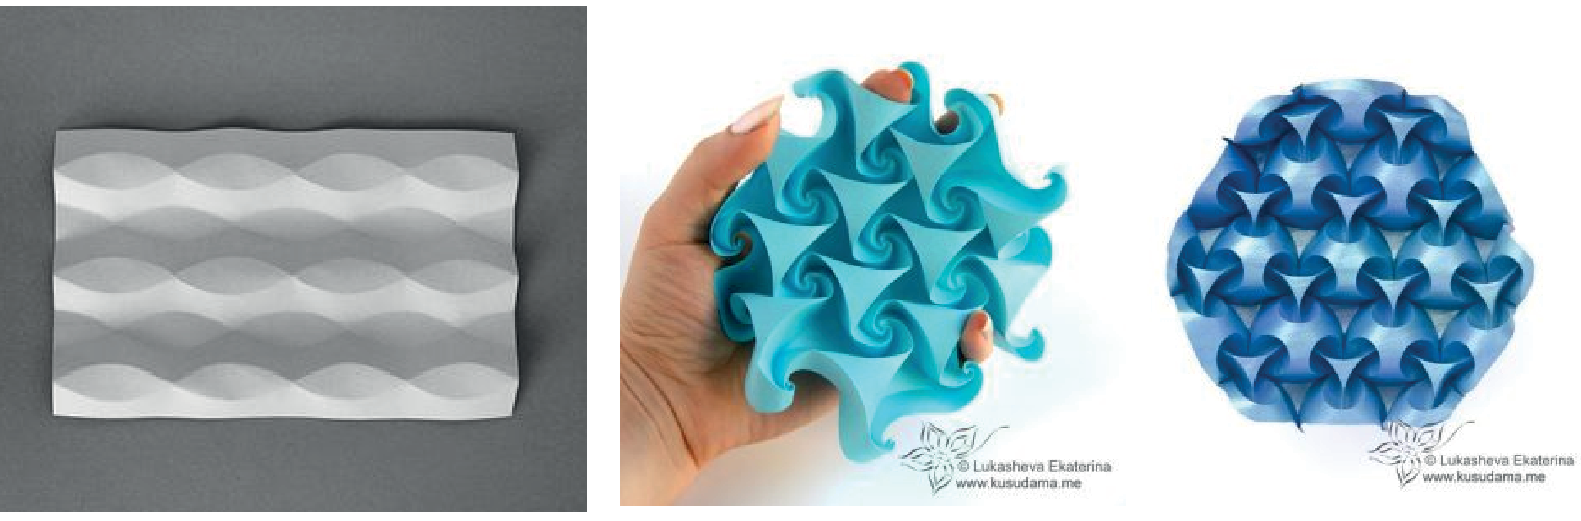
\includegraphics[width=\linewidth]{figures/curved_wallpapers}
  \caption{\label{fig:curved_wallpapers_teaser} \MiR{replace with teaser, most likely also wallpaper.}
}
\end{teaserfigure}
\begin{abstract}
% !TEX root =  CurvedFoldedDogs.tex
We present a computational framework for interactive design and exploration of curved folded surfaces. In current practice, such surfaces are typically created manually using physical paper, and hence our objective is to lay the foundations for the digitalization of curved folded surface design. 
Our main contribution is a discrete binary characterization for folds between discrete developable surfaces, accompanied by an algorithm to simultaneously fold creases and smoothly bend planar sheets. We complement our algorithm with essential building blocks for curved folding deformations: objectives to control dihedral angles and mountain-valley assignments. We apply our machinery to build the first interactive freeform editing tool capable of modeling bending and folding of complicated crease patterns.



%We base our approach on modeling the shapes using discrete orthogonal geodesic nets (DOGs) in a piecewise manner. DOGs are used to represent the smooth parts of the modeled shape, and we connect different DOGs along curves that represent the sharp creases and folds.
%Our main contribution is a discrete binary characterization for folds between DOGs, accompanied by an algorithm to simultaneously fold creases and smoothly bend planar sheets. We complement our algorithm with essential building blocks for curved folding deformations: objectives to control dihedral angles and mountain-valley assignments. We apply our machinery to build the first interactive freeform editing tool capable of modeling bending and folding
%of complicated crease patterns.
\end{abstract}


%
% The code below should be generated by the tool at
% http://dl.acm.org/ccs.cfm
% Please copy and paste the code instead of the example below.
%
\begin{CCSXML}
<ccs2012>
<concept>
<concept_id>10010147.10010371.10010396.10010397</concept_id>
<concept_desc>Computing methodologies~Mesh models</concept_desc>
<concept_significance>500</concept_significance>
</concept>
<concept>
<concept_id>10010147.10010371.10010396.10010398</concept_id>
<concept_desc>Computing methodologies~Mesh geometry models</concept_desc>
<concept_significance>500</concept_significance>
</concept>
</ccs2012>
\end{CCSXML}

\ccsdesc[500]{Computing methodologies~Mesh models}
\ccsdesc[500]{Computing methodologies~Mesh geometry models}

%
% End generated code
%


\keywords{curved folding, developable surfaces, discrete differential geometry, geodesic nets, shape modeling}



\maketitle
% !TEX root =  CurvedFoldedDogs.tex


\section{Introduction}
There are infinitely many ways to deform a planar sheet without stretching or tearing it. One can either bend it, form sharp creases by folding it, or combine the two. Folding and bending isometries are different by nature, and historically there has been a dichotomy in the study of the two. Smooth bending deformations are typically studied in differential geometry \cite{do_carmo}, whereas straight folds are  explored in the field of computational origami \cite{origami_book}. Curved folded surfaces \cite{huffman} (\figref{fig:teaser}) can be viewed as a combination of the two, since folding an inextensible sheet along a curve necessitates global bending around the crease. These elegant geometries have garnered the attention of architects, artists, and industrial designers \cite{arch_geom,tachi2013composite,tachi2011one,buri2011curved,robofold,curved_review}.

The design of a curved folded surface is manual and time consuming and is usually done using an empirical trial and error approach \cite{curved_review,huffmann_reconstructing}. The known theory on curved folds is confined to a narrow set of folds, and contrary to classical origami, bending and folding instructions are hard to write down and multiple creases must be folded simultaneously \cite{StringActuated:2017}. Artists generally pre-crease the paper using a ball burnisher or a CNC plotter before carefully folding and bending, making the process of shape exploration even slower. 

Although manual and slow, playing with paper is still the predominant approach for curved folded surface design. Existing works on modeling such surfaces are either limited to previously discovered surfaces \cite{curved_folding_kilian,StringActuated:2017} or model a small, partial set of folded surfaces generated by reflections or rotational sweeps \cite{Mitani_ref,mitani2009design}. Modeling the folding process of novel forms remains a challenge \cite{curved_review}. 

In this paper we set out to develop the basic tools for freeform modeling of curved folds, with the objective of aiding the exploration, analysis and study of new curved folded surfaces. Our work builds upon discrete orthogonal geodesic nets (DOGs) \cite{rabi18,rabi2018shape} as a discrete model for $C^2$ developable surfaces. DOGs are regular quadrilateral meshes where around each vertex all angles are equal. Unlike other computational models for developable surfaces, DOGs do not suffer from locking of various deformation modes \cite{locking1,locking2,grin_shells}, \newt{are not limited by an initial choice of meshing or rulings} \cite{pottmann_new,curved_folding_kilian,stein_dev,solomon} (see \figref{fig:rulings_problem_curve}) and do not require remeshing while deforming the surface \cite{StringActuated:2017,SchreckEG2017,Narain}. \newt{Therefore DOGs are particularly suited for modeling curved folds.}
Given an input crease pattern, we represent a curved folded model as a collection of DOGs, with boundary constraints enforcing equal discrete geodesic curvature along their intersections, as done in \cite{rabi2018shape}.

In practice, deforming a set of DOGs while keeping the geodesic boundary constraints does not usually result in a model that is folded along all creases (see \figref{fig:folded_and_not_folded}). Part of the difficulty of modeling these deformations stems from the need to fold all curves simultaneously starting from a flat configuration. \newt{The primary goal of our work is to deal with this difficulty.} 

\subsection{\newt{Contributions}}
\begin{itemize}[label={--}]
  \item \newt{We present a discrete binary characterization for folds between discrete developable surfaces based on supporting planes along creases, motivated by a novel analysis on curved folded surfaces.}
  \item \newt{We use the previous derivation to devise an optimization algorithm capable of enforcing folds while deforming a piecewise DOG, without requiring any folding angles or mountain/valley assignments as input.}
  \item \newt{We further derive optional objectives to control dihedral angles and mountain/valley assignments along folds.}
\end{itemize}
\newt{Though we use DOGs as an underlying model for developable surfaces, our work and derivations can be applied on top of other discrete models for developable surfaces such as the models of \cite{grin_shells,conical}.}

%In practice, deforming this set of DOGs while keeping the geodesic boundary constraints does not usually result in a model that is folded along all creases (see \figref{fig:folded_and_not_folded}). Our primary goal is to study deformations that bend as well as \emph{fold} along all creases. Part of the difficulty of modeling these deformations stems from the need to fold all curves simultaneously starting from a flat configuration. \secref{sec:setup} lays the setup for our work, including the problem definition, desiderata and the discrete model we build upon (taken from \cite{rabi18,rabi2018shape}). In \secref{sec:folding} we look at the continuous and combinatorial degrees of freedom of curved foldings, detailing how a flat piecewise smooth developable surface is locally a bifurcation point between folded and unfolded configurations. We discuss how folding along a crease given one side of the surface is a binary choice (see \figref{fig:folding_combinatorics}), give a simple discrete characterization for this choice by looking at supporting planes along the crease and derive objectives to control the basic properties of folding: dihedral angles and mountain/valley assignments. In \secref{sec:implementation} we translate these derivations into an optimization algorithm capable of enforcing folds while deforming a piecewise DOG. Finally, in \secref{sec:results} we model various curved folded surfaces.

\begin{figure} [t]
	\centering
	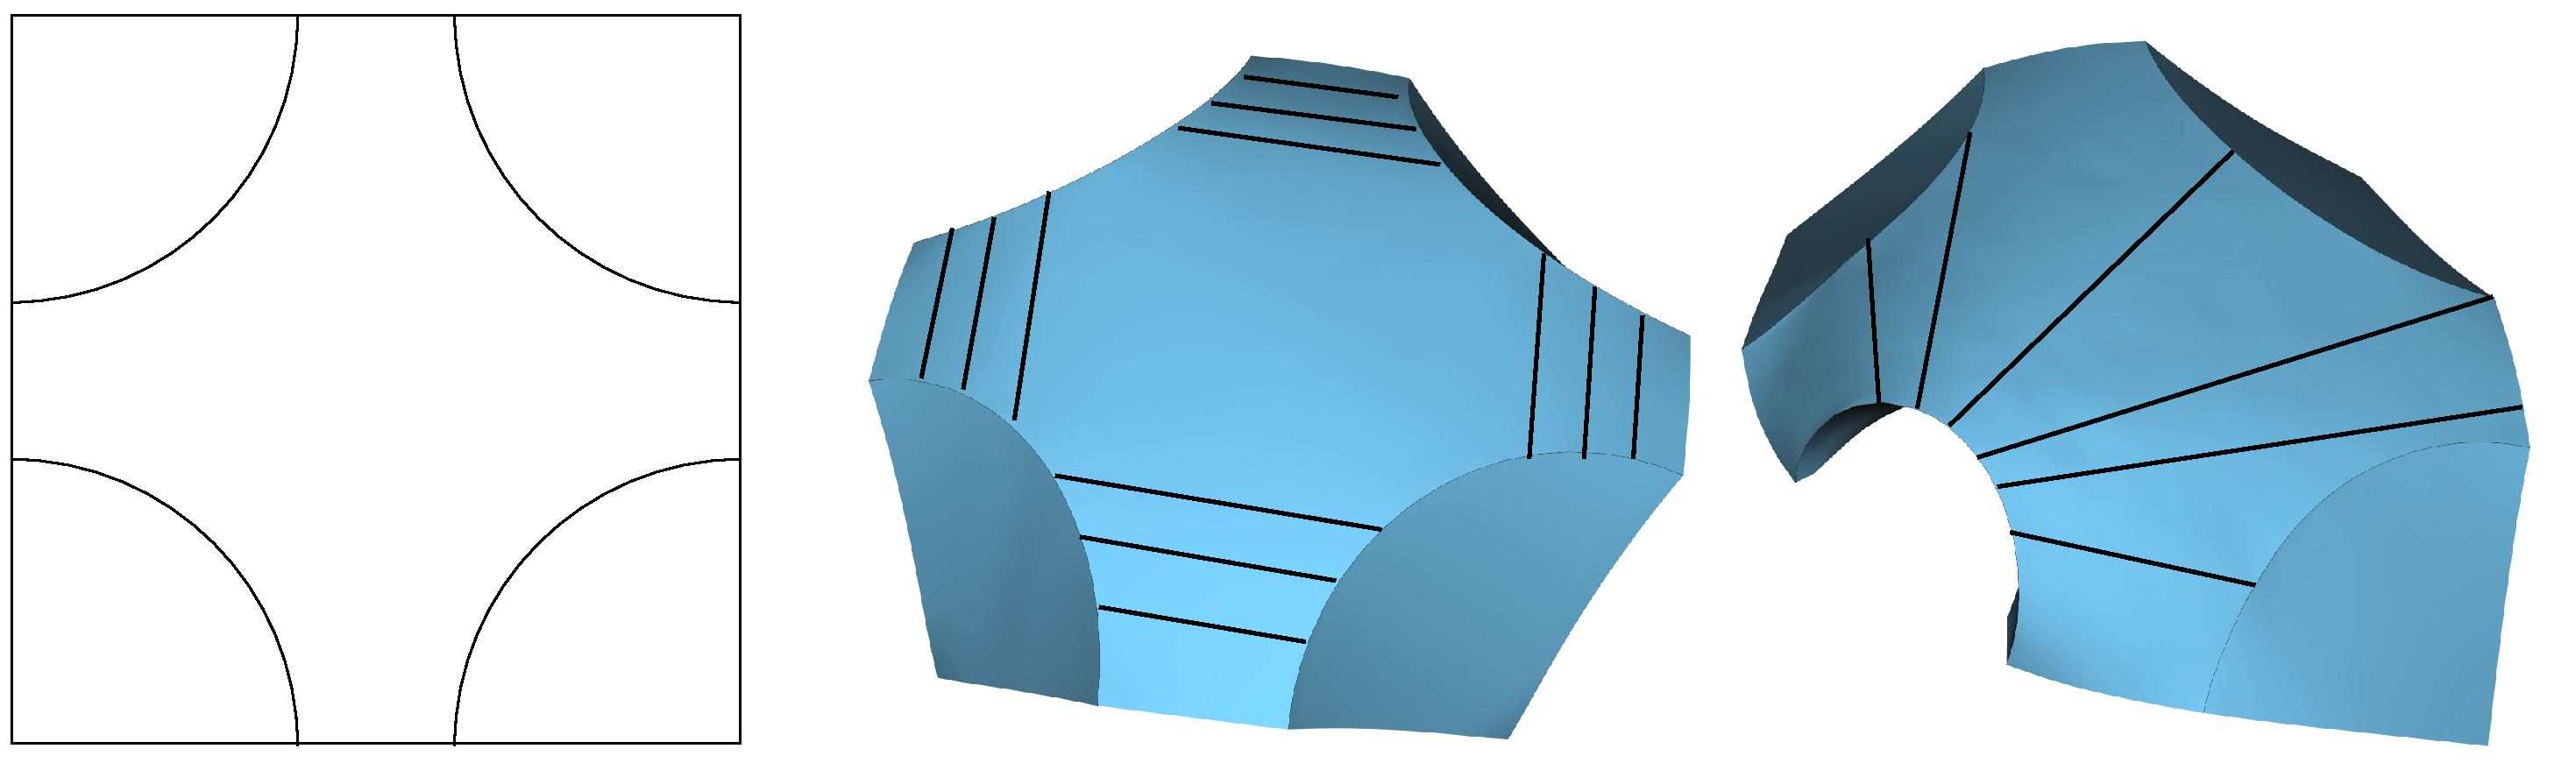
\includegraphics[width=\linewidth]{figures/rulings_problem_curve}
	\caption{Folding and bending the same curved crease pattern (left) into two different surfaces, with some of their rulings plotted. Methods that model the rulings explicitly must remesh in order to model these surfaces, since the rulings can change drastically, connecting vertices of different patches to one another. Representing the curved folded surface as a piecewise DOG avoids the need to remesh because a DOG is parameterized by intrinsic invariants -- orthogonal geodesics -- and does not explicitly encode the developable rulings in its mesh.}
	\label{fig:rulings_problem_curve}
\end{figure}

\begin{figure*} [h]
	\centering
	\includegraphics[width=\linewidth]{figures/fold_bias_compare}
	\caption{Comparison of the same deformation objective with and without our folding algorithm. Up: Crease patterns given as input. Center: Applying a positional based deformation objective of the crease patterns without our folding algorithm results in most crease curves being ignored, i.e. not folded. At this stage, one cannot bend these creases without first flattening the surface. Down: Result of applying the same deformation with our folding algorithm. Our folding algorithm simultaneously folds all crease points while deforming a surface by adding a bias that effectively push flat points towards a folded configuration while not affecting already folded points. The crease mountain/valley assignments, which in these examples are in fact fixed given one choice, are determined automatically without any input. The objective of all of these deformations were the same positional constraints defined on mesh vertices or on a part of a crease curve based on a \textit{curve-constraining flow} \cite{rabi2018shape}.}
	\label{fig:folded_and_not_folded}
\end{figure*}
\section{Related work}
\subsection{Modeling developable surfaces}
A smooth surface is called a \textit{developable surface} if it is locally isometric to the plane, or equivalently has zero Gaussian curvature. Though well understood mathematically \cite{do_carmo,spivak,computational_line}, there is a plethora of work on modeling developable surfaces, which has been proven to be a challenge. The primary difficulty lies in using a discrete model that is able to capture the full set of deformations keeping a surface developable. These include extrinsic deformations as well as intrinsic deformations. The latter stretch the surface while keeping it developable, and is used for geometry exploration tasks where the size and shape of the flattened developable surface is unknown \cite{conical,pottmann_new,rabi2018shape}. A failure of a discrete model to discretize the full range of smooth deformations is often termed \textit{locking} \cite{solomon,locking1}. Ruling based discrete models \cite{conical,curved_folding_kilian,pottmann_new,stein_dev} lock the user to a partial set of extrinsic deformations while isometry based simulations \cite{grin_shells,shells, goldenthal2007efficient,froh_botsch} do not model intrinsic deformations by design, but are also prone to locking of various bending deformations \cite{locking1,locking2}, and is often coupled with dynamic remeshing \cite{narain2012adaptive,StringActuated:2017,Narain,SchreckEG2017}. \MiR{should I explicitly say that remeshing is complicated and is also not backed up by any theory?}
\subsection{Curved folding}
%The beautiful art of curved folded sculptures is almost a hundred years old, dating back to the 1920's works of Josef Albers in the Bauhaus art school \cite{josef_albers_thesis}, and continuing with the investigations of David Huffman and Ron Resch in the 1970's \cite{huffman,resch1974portfolio}. Many of these early works are mathematically not yet fully understood. %TODO. (some work has been done on specific models...$

%  We know what happens in one fold, but multiple ones still forms a challenge and we only have specific investigation for some cases. Creating them is , using paper and They date to 1920's but we only know what happen along one fold, or analyze specific set of examples, and don't know how typical models even fold. Computer simulations of that can help, but are somehow legging behind what is mostly experimented by hand, in a process that is in fact time consuming, often involving using a pen bla and da da da.
\section{Setup} \label{sec:setup}
\subsection{Definitions}
Throughout the paper, we use the following definition for a curved folded surface:
\begin{definition} \label{def:curved_folded_surface}
A surface $S$ is called a curved folded surface if it is locally isometric to the plane and can be written as $S = \bigcup P_i $ where each $P_i$ is a $C^2$ developable surfaces termed a \textit{patch}, and their intersections $P_i \cap P_j$ are $C^2$ curves.
\end{definition}
% consists piecewise $C^2$ developable surface whose discontinuities are focused along $C^2$ curves. More formally, 
This definition is suitable for various topologies, such as a cylinder, although throughout the paper we will work with surfaces that can be globally isometrically flattened to the plane. Borrowing terms from \cite{origami_book,non_pleated}, we often refer to the surface \textit{crease pattern} consisting of the planar isometric surface domain $S_P$ together with the flattened intersection curves between the interior of the patches $P_i$ (see \figref{fig:crease_pattern}). Flattened creases with non zero curvature are said to be curved while those with zero curvature are said to be straight. A crease might be partly curved and partly straight, or a mostly curved but with an inflection point where the curvature vanishes. When we discuss curved folds we always assume non-zero curvature, unless specified otherwise. The flattened domain boundaries together with the flattened intersection curves form a (pseudoline) planar arrangement \cite{arrangements}, inducing a planar graph decomposing $S_p$ into different disconnected components termed faces, which are domains isometric to the patches $P_i$. The vertices of this graph are the intersection of the curves with each other or the boundary curves, which we call \textit{crease vertices}. The \textit{edges} of this graph are curves isometric to the intersections of the various patches (see \figref{fig:crease_pattern}), and we refer to the inner points of these curves as \textit{crease points}, i.e. points on these curves that are not \textit{crease vertices}. We say that $S$ is \emph{folded} along a crease point if at that point the patches $P_i,P_j$ sharing it have a tangential discontinuity (see \figref{fig:folded_and_not_folded}).

\begin{figure} [h]
	\centering
	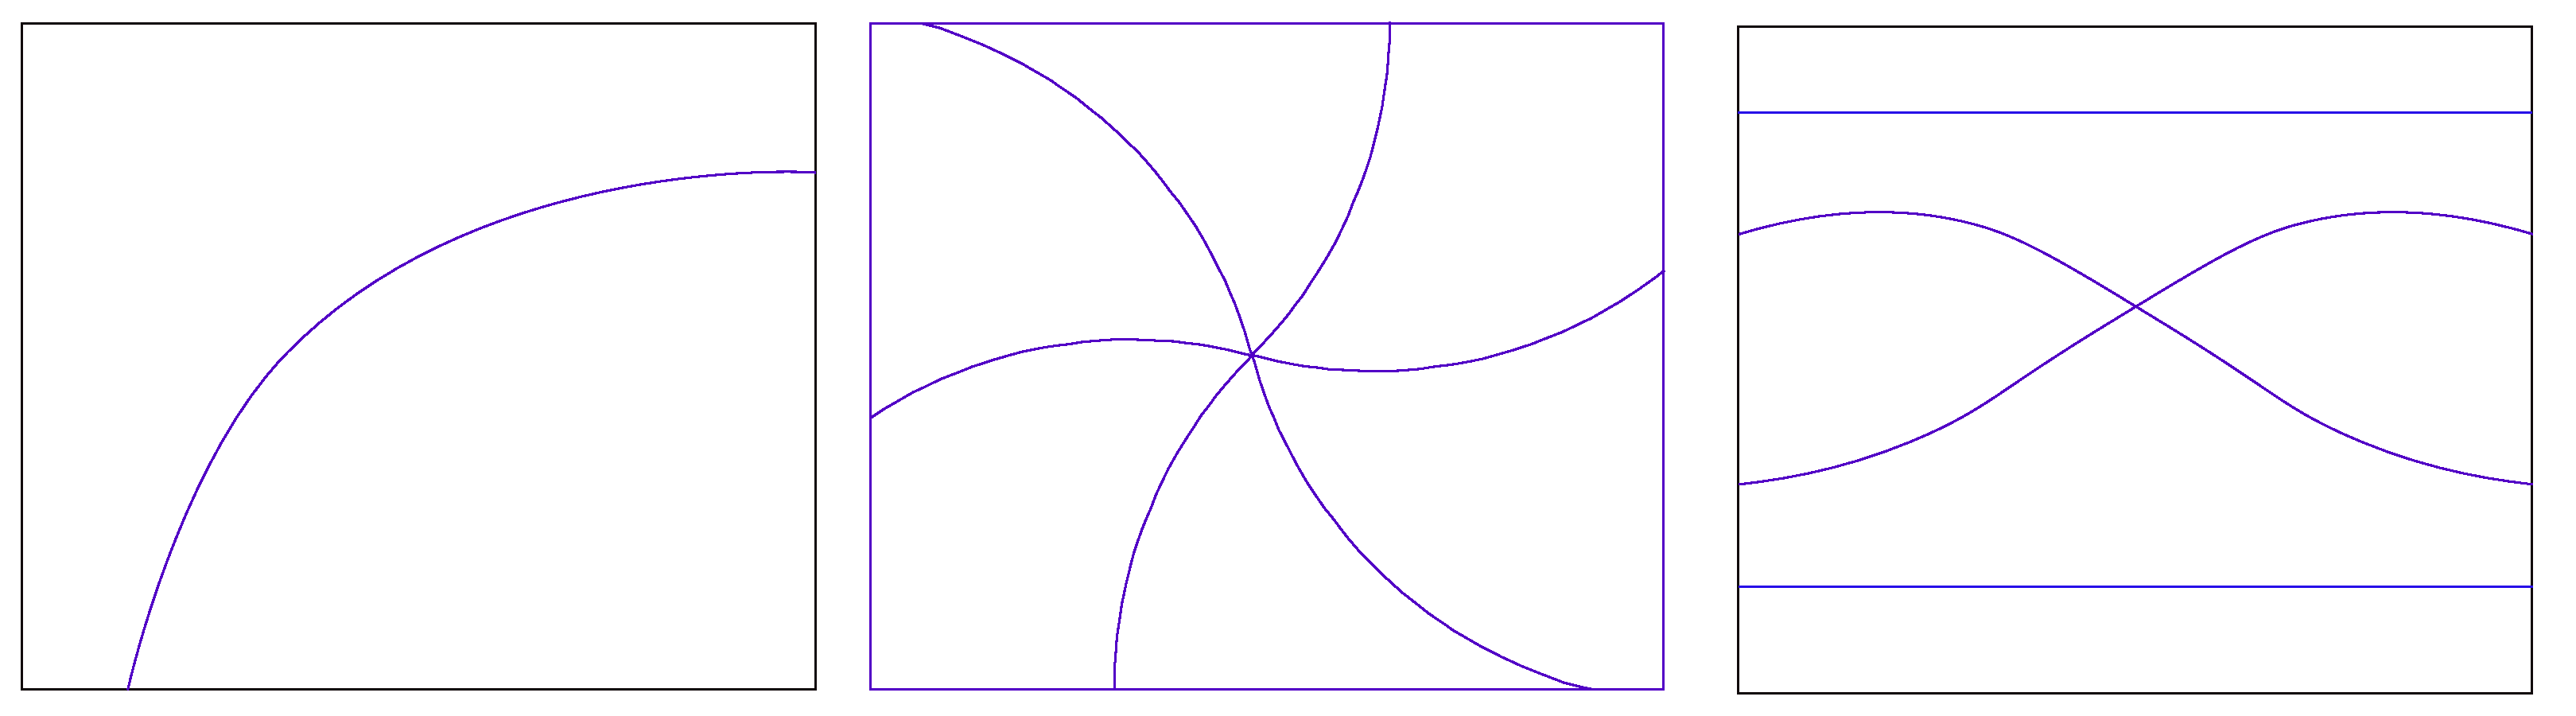
\includegraphics[width=\linewidth]{figures/crease_patterns}
	\caption{Curved crease patterns, decomposing a pattern into multiple components $P_i$ and intersecting at crease vertices. Boundary curves in black, crease curves in blue.}
	\label{fig:crease_pattern}
\end{figure}
We are interested in deformations on curved folded surfaces that keeps them curved folded. Viewed separately on each patch $P_i$, these deformation are $C^2$, though they often introduce tangent discontinuities along the patches intersections. At \cite{demaine_lens} the authors refer to creases that remain $C^2$ as \textit{smoothly folded} creases (though they define it as $C^1$ they prove that this implies that they are $C^2$). In particular we are interested in such continuous deformations, or deformation flows \cite{rabi2018shape}, which we refer to as curved folding flows. We denote these flows by a continuous map $S(t), 0 \leq t \leq 1$, where each $S(t)$ is a curved folded surface and the flow is $C^2$ when limited to each patch. We often look at the case where the starting point $S(0)$ planar. In this paper we focus on modeling isometric curved flows, which we also refer to as \emph{folding}. These flows can can be used to model physical paper or metal folding, though most of our observations and tools can also be used to model curved folding flows that are not isometries. Non-isometric developable deformations can be useful for design tasks where the a-priori flattened shape is unknown \cite{rabi18,rabi2018shape} .

\subsection{Model} \label{sec:model}
We follow the work of \cite{rabi2018shape} by modeling each patch $P_i$ as a discrete orthogonal geodesic net (see \figref{fig:curve_on_dog}). We represent a crease as piecewise linear curves, whose points $c(i)$ are represented by the curves' intersection point with the grid edges. Each point $c(i)$ is a linear combination of two vertices on a DOG: $c(i) = t_i v_k + (1-t_i)v_j,$ where $0 \leq t_i \leq 1$ and $v_k,v_j$ are too neighbour vertices on the grid.  Each point on a crease lies on each of the $m \geq 2$ different patches, essentially duplicated. If $c(i)^1,c(i)^2,....,c(i)^m$ are the representation of $c(i)$ on the different patches, we enforce constrain these duplicated points have equal coordinates (see \figref{fig:curve_on_dog}).
We trivially extend the represntation at \cite{rabi2018shape} to support intersecting curves by adding grid lines at crease vertices (see \figref{fig:piecewise_dog_from_crease} and \figref{fig:curve_on_dog}).

\begin{figure} [h]
	\centering
	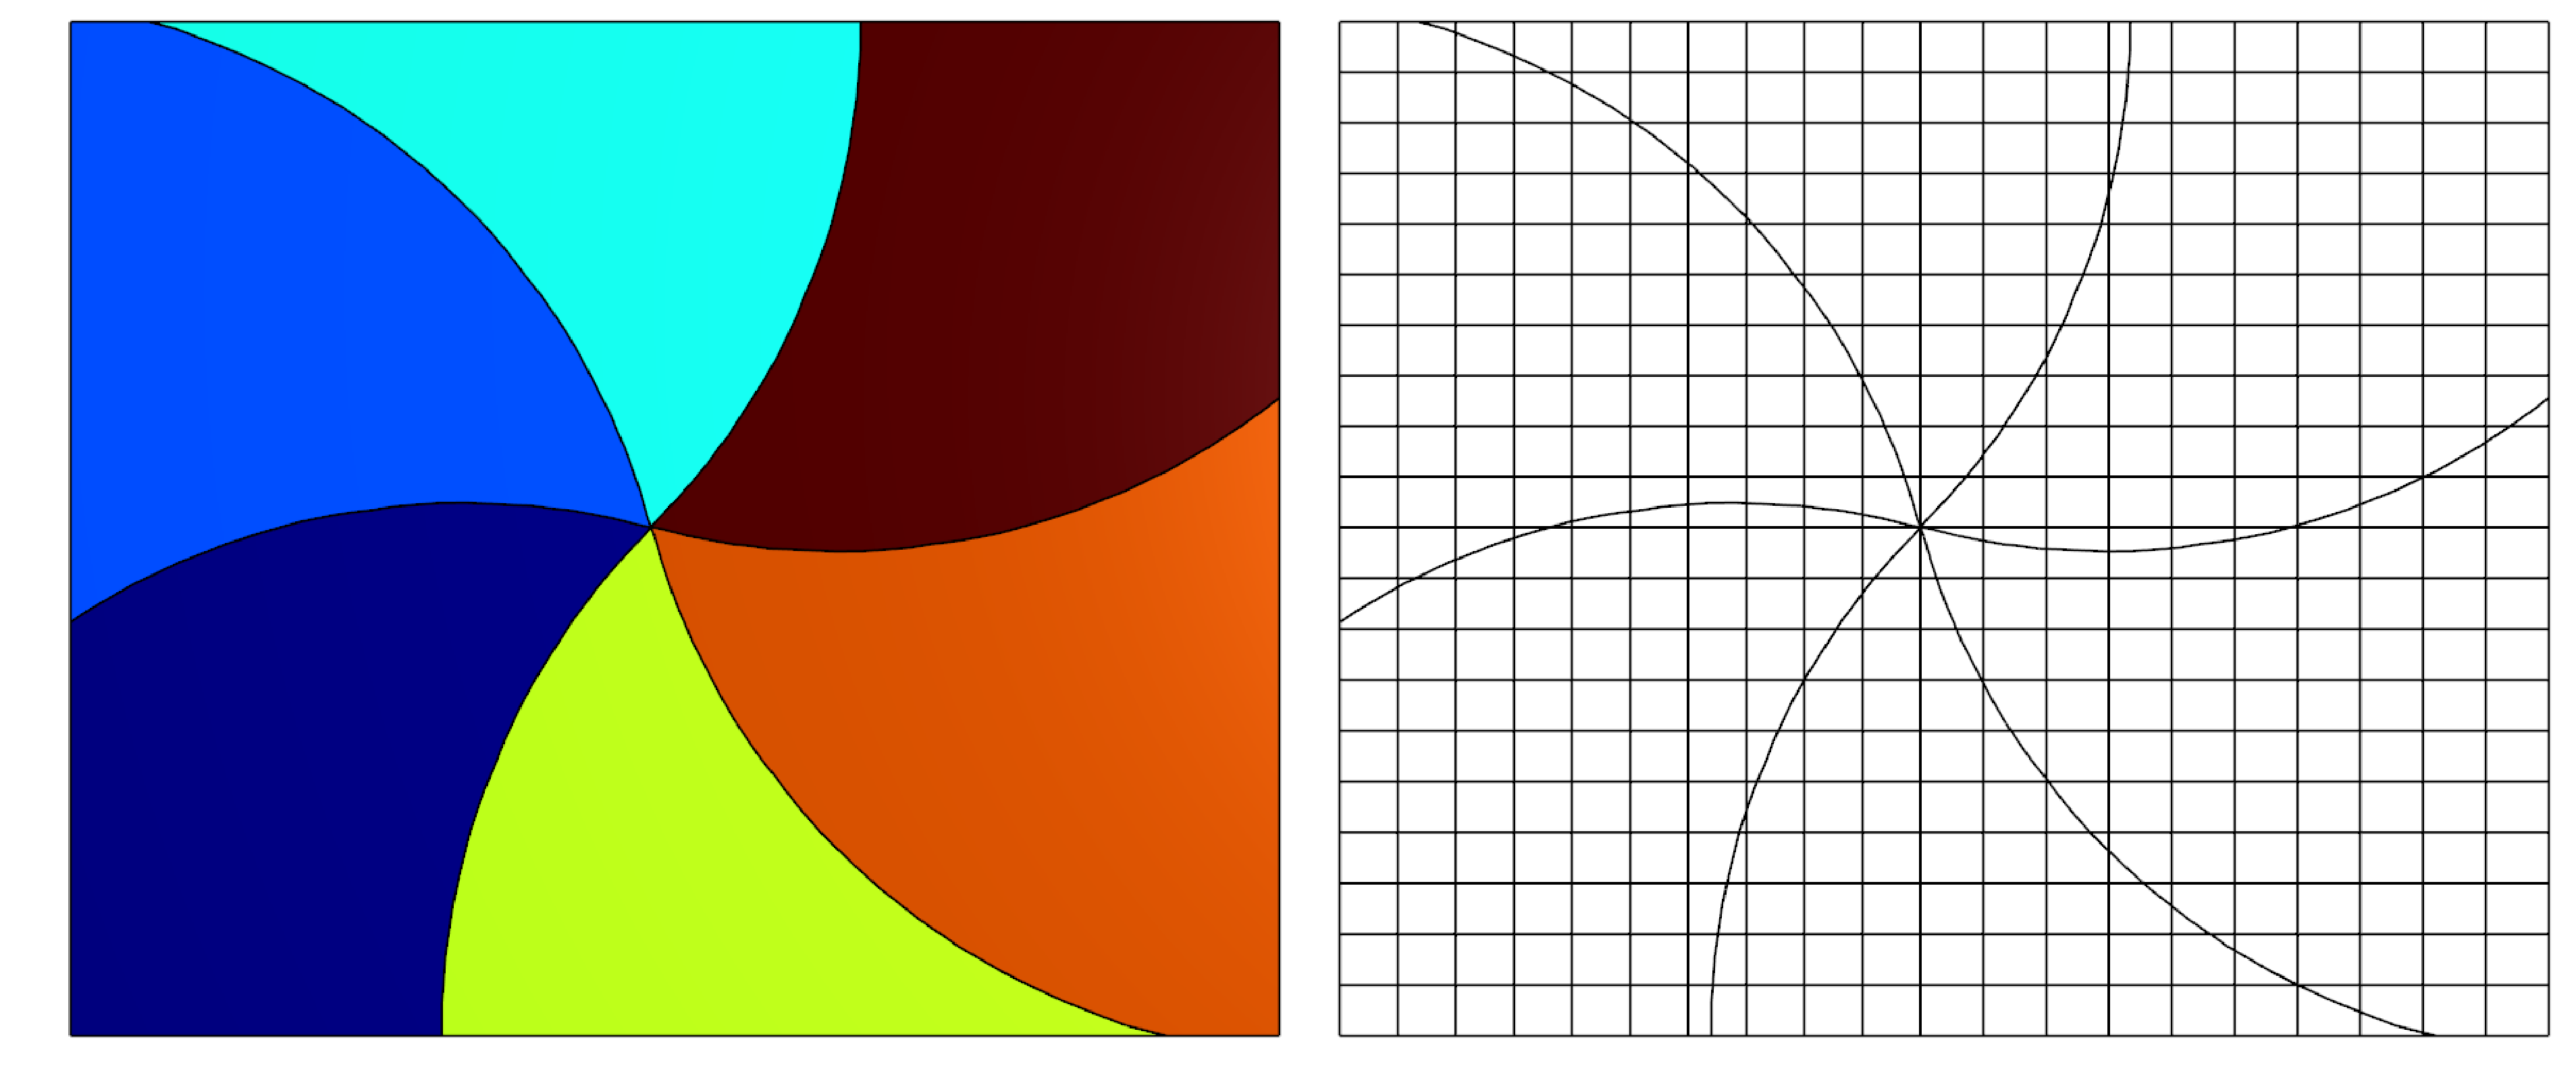
\includegraphics[width=0.8\linewidth]{figures/piecewise_dog_from_crease}
	\caption{Given a crease pattern, we create a DOG for each segment (colored differently), and use the boundary constraints as done in \cite{rabi2018shape}.}
	\label{fig:piecewise_dog_from_crease}
\end{figure}

\begin{figure} [h]
	\centering
	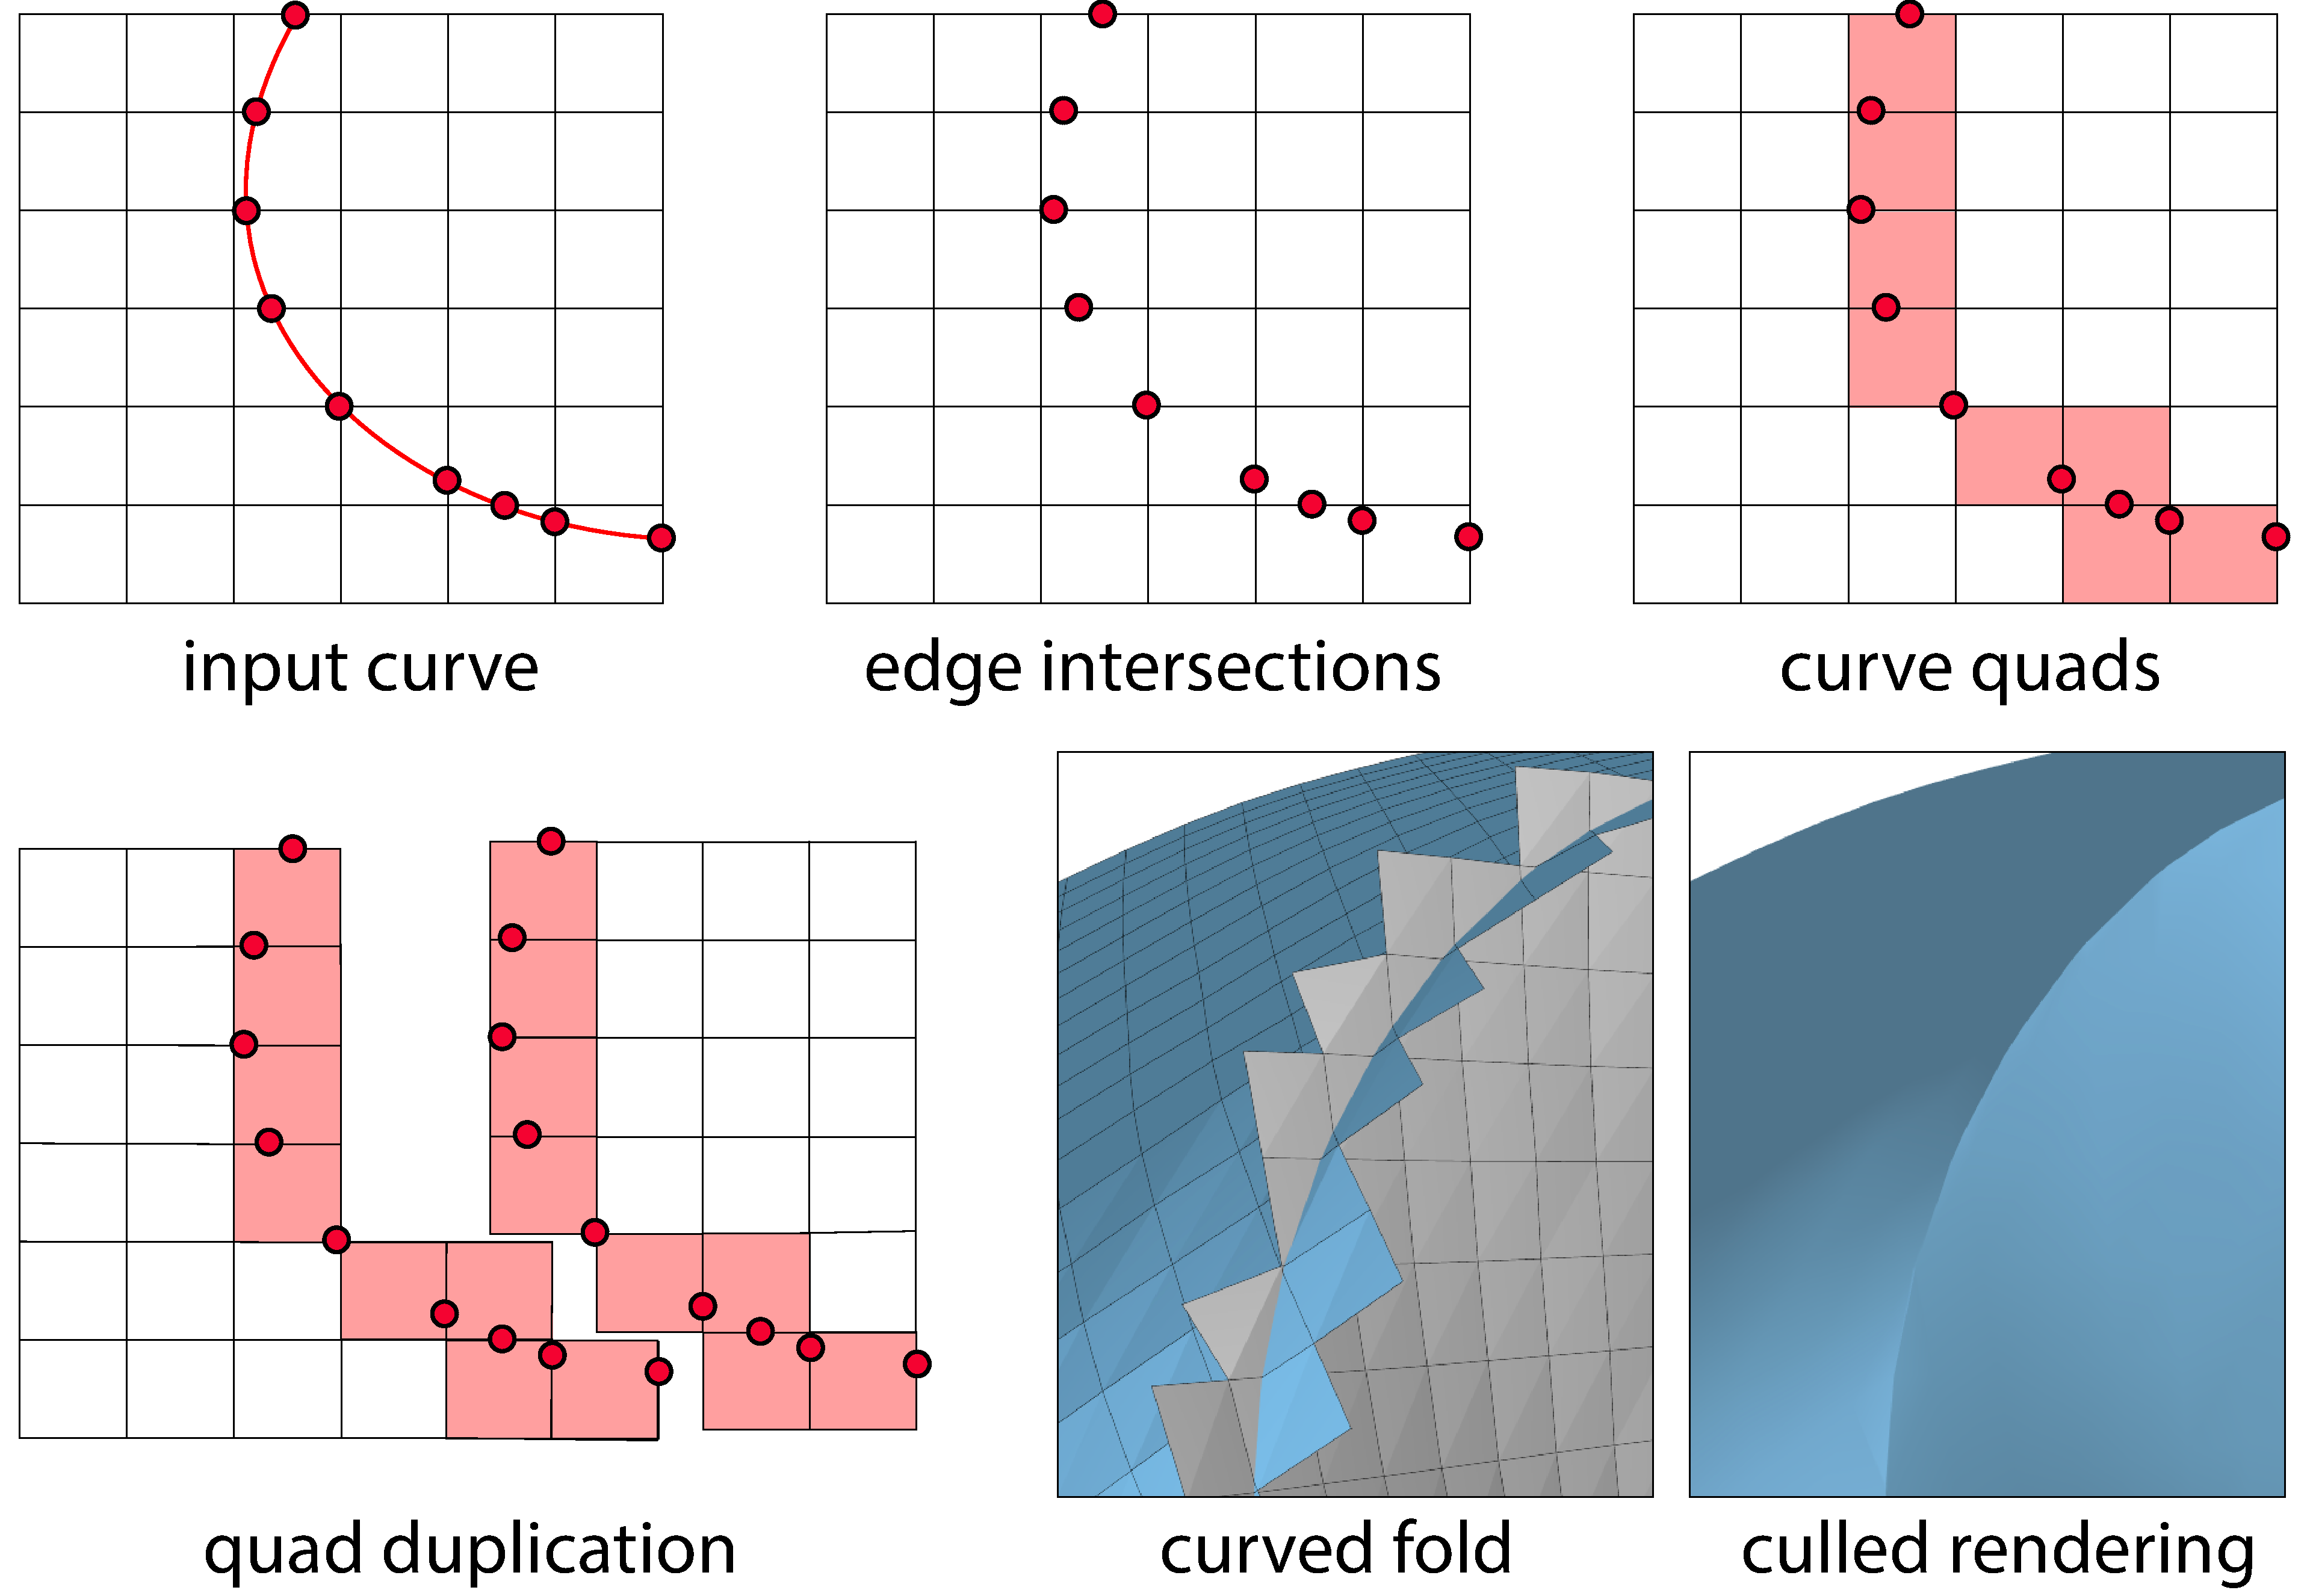
\includegraphics[width=0.8\linewidth]{figures/curve_on_dog}
	\caption{Picture taken from \cite{rabi2018shape}.}
	\label{fig:curve_on_dog}
\end{figure}

\subsection{Desiderata}
Our goal is to develop tools for the exploration of curved folded shapes on top of piecewise DOGs by means of deformations. Our choices are guided by the following ground rules for deforming DOGs:
\begin{enumerate}
  \item Perform homotopy based optimization \label{homotopy_opt}
  \item Minimally constrain DOGs \label{minimal_const}
%  \item Use accurate functionals \label{accurate_func}
%  \item Use simple functionals
\end{enumerate}
\textbf{Homotopy based optimization} is motivated both theoretically and empirically; Modeling DOGs requires solving highly constrained and non linear optimization problems, yet the theory of DOGs guarantees the existence of nearby solutions if one starts at a feasible point. In fact, generally the shape space of DOGs is a smooth manifold \cite{rabi2018shape}. This observation is worthwhile in practice; DOGs exploration was demonstrated to perform well using smooth flow, or homotopy based optimization methods both for handle based editing tasks as well for more complicated deformations such as curve-constraining flows \cite{rabi2018shape}. \\
\textbf{Minimally constrain DOGs.} As DOGs are already heavily constrained, one needs to carefully choose which quantities to constrain by hard constraints, and which ones should be optimized using soft constraints. This is essential to avoid locking, or ill-posed problems in case the constraint gradients are linearly independent \cite{rabi2018shape}. In particular, the rigidity analysis in \cite{rabi18} demonstrates that one cannot fix all edge length exactly, or likewise demand a DOG to also be a Chebyshev net. We note however that this can be done approximately and to a low tolerance as a DOG is a chebyshev at the smooth limit and at the smooth limit there is a rich set of exact isometries. The folding constraints at \secref{sec:folding} where chosen such that they could be satisfied \textit{exactly}, and so that in practice they vanish once the surface is sufficiently folded, just like a piecewise smooth curved folded surface. \\
%\textbf{Accurate functionals.} We look for constraints and objectives that are accurate and as often in the case with DOG objectives, converge under sampling of a smooth orthogonal geodesic net \cite{rabi18,rabi2018shape}. \\
%\textbf{Simple functionals.} We strongly prefer sparser objectives with a lower degree as possible. To that end, we leverage the regularity of the DOG meshing and theory on smooth orthogonal geodesic nets in our derivations. \\
% !TEX root =  CurvedFoldedDogs.tex

\section{Folding crease patterns} \label{sec:folding}
In this section we explore the different ways one can fold a given crease pattern. Our result is a discrete combinatorial characterization for the local existence of a fold in a piecewise DOG.

%Two intersecting developable surfaces can be flattened along their intersection if the intersected curve have the same geodesic curvature on both surfaces. 
\subsection{The smooth and combinatorial degrees of freedom around a single curved crease}
\label{sec:smooth-combinatorial}

Straight creases are rather boring, mathematically speaking. Straight lines can only be folded as in classical origami, i.e., by keeping them straight \cite{demaine_lens}, unless one first folds a crease by $180$ degrees, such that the two incident sheets coincide. Hence a folding of a single straight crease can be described by a single real number representing the constant dihedral angle between the incident planes. There are infinitely many ways, or degrees of freedom, to fold a curved crease. If $S$ is a surface with a folded crease, and $P$ is its flattened isometric reference, then one can locally deform the curved surface $S$ by freely deforming the crease curve, as long as the absolute value of the crease curvature stays greater than its flattened curvature in $P$ \cite{more_on_paper}. Up to a rigid motion, a curve is defined by its curvature and torsion functions.

One can flip this point of view: Given a planar domain $P$, a curve on the domain $\gamma(t)$ and a deformed, isometric space curve $\Gamma(t)$ with greater absolute curvature than that of $\gamma(t)$, there are only two smooth surfaces isometric to $P$ passing through $\Gamma(t)$ such that the unfolding of the surface to the plane maps $\Gamma(t)$ to $\gamma(t)$ \cite{mathematical_omnibus} (see \figref{fig:folding_combinatorics} left and center).


%To see that, assume that $S$ is such a surface; assume a crease pattern consisting of a single crease such that $S = P_1 \cup P_2$ (\figref{fig:folding_combinatorics} left). Let $\Gamma(t) = P_1 \cap P_2$ be the 3D crease curve and $\gamma(t)$ its flattening in $P$. Let $\kappa(t)$ be the curvature of $\Gamma(t)$ and $\kappa_g(t) = \kappa(t) \cos(\alpha(t))$ be its geodesic curvature \OSH{who is $\alpha(t)$?}. Assume that the curve is bent further in space, i.e., $\kappa(t) > \kappa_g(t)$. Then the tangent planes of $P_1$ and $P_2$ form an angle of $2\alpha(t) \neq 0$ with the osculating plane of $\Gamma(t)$ \cite{more_on_paper,duncan_folded}. Since $P_1,P_2$ are $C^2$,  there are four options for a consistent choice of a family of tangent planes along each side of the crease $\Gamma(t)$. Two of these four options correspond to a folding (i.e., tangent discontinuity) by choosing one family tangent planes along $\Gamma(t)$ for $P_1$ and the other for $P_2$ (see \figref{fig:folding_combinatorics}).
\begin{figure} [t]
	\centering
	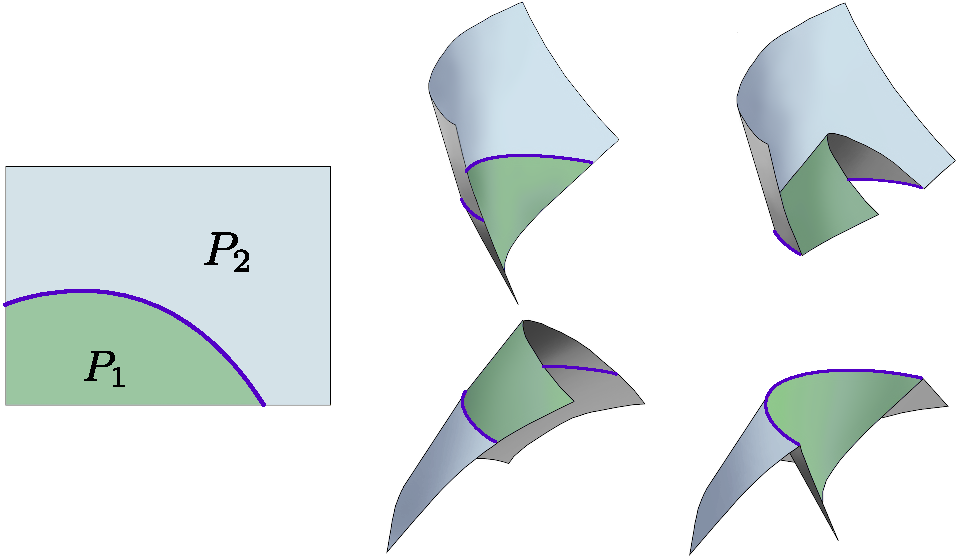
\includegraphics[width=\linewidth]{figures/curved_fold_through_curve_1.pdf}
	\caption{Illustration of the combinatorial degrees of freedom in curved folding. If a crease pattern of a curved folded surface (left) is isometrically folded such that a given curve lies in some configuration in $\R^3$, then there are only two smooth surfaces that isometrically flatten into the crease pattern (center). One can also choose a different surface for each patch $P_1,P_2$, resulting in two other, curved folded surfaces (right).}
	\label{fig:folding_combinatorics}
\end{figure}

If one permits the surface $S$ to have a fold along $\Gamma(t)$ but remain smooth around it, then there are four possible surfaces: two of them are smooth, while the other two are folded along the curve (see \figref{fig:folding_combinatorics}). If $S = S_1 \cup S_2$ is folded along $\Gamma(t) = S_1 \cap S_2$ then the angle between the tangent planes of $S_1,S_2$ along the curve is called the folding angle, which we denote by $\theta(t) > 0$. Unlike the case of a straight crease, $\theta(t)$ often varies along the curve.  The bigger the curvature of $\Gamma(t)$, the bigger the folding angle. If $\kappa(t)$ is the curvature of the space curve $\Gamma(t)$, $\kappa_g(t)$ is its geodesic curvature, which is also the curvature of $\gamma(t)$, then $\kappa_g(t) = \kappa(t) \cos\frac{\theta(t)}{2},$ implying that the osculating plane of the crease $\Gamma(t)$ bisects the tangent planes of the smooth patches intersecting at $\Gamma(t)$ \cite{curved_folding_kilian,duncan_folded}. The folding angle does not dictate the shape of the surface, as different surfaces can be generated with the same $\theta(t)$ by varying the torsion of $\Gamma(t)$, thereby changing the ruling pattern of each developable patch. The connection between $\theta(t)$, the curvature and the torsion of $\Gamma(t)$, the curvature of $\gamma(t)$ and the rulings of each incident patch is further detailed in \cite{demaine2018conic}.

To summarize, the shape of a curved folded surface $S$ with a single curved crease $\Gamma(t)$ can be locally described by two {real functions} for the curvature and torsion of $\Gamma(t)$ under the condition of sufficient absolute curvature, as well as an additional combinatorial parameter distinguishing between four possible surfaces, two of which have a fold.
 
\subsection{The combinatorial parameters of multiple creases}
The previous analysis explains the local behavior of curved folding around a single curve. Understanding crease patterns globally still remains a challenge. In essence, deforming one patch propagates a global deformation of the patch on the other side of the crease, a process that depends on the locations of the creases and the possibly changing ruling lines along the developable. When there are multiple creases, the propagation dictates the shape of other patches. The process becomes more complicated when some creases intersect, due to compatibility constraints (see \figref{fig:multiple_crease_patterns}). 

\begin{figure} [t]
	\centering
	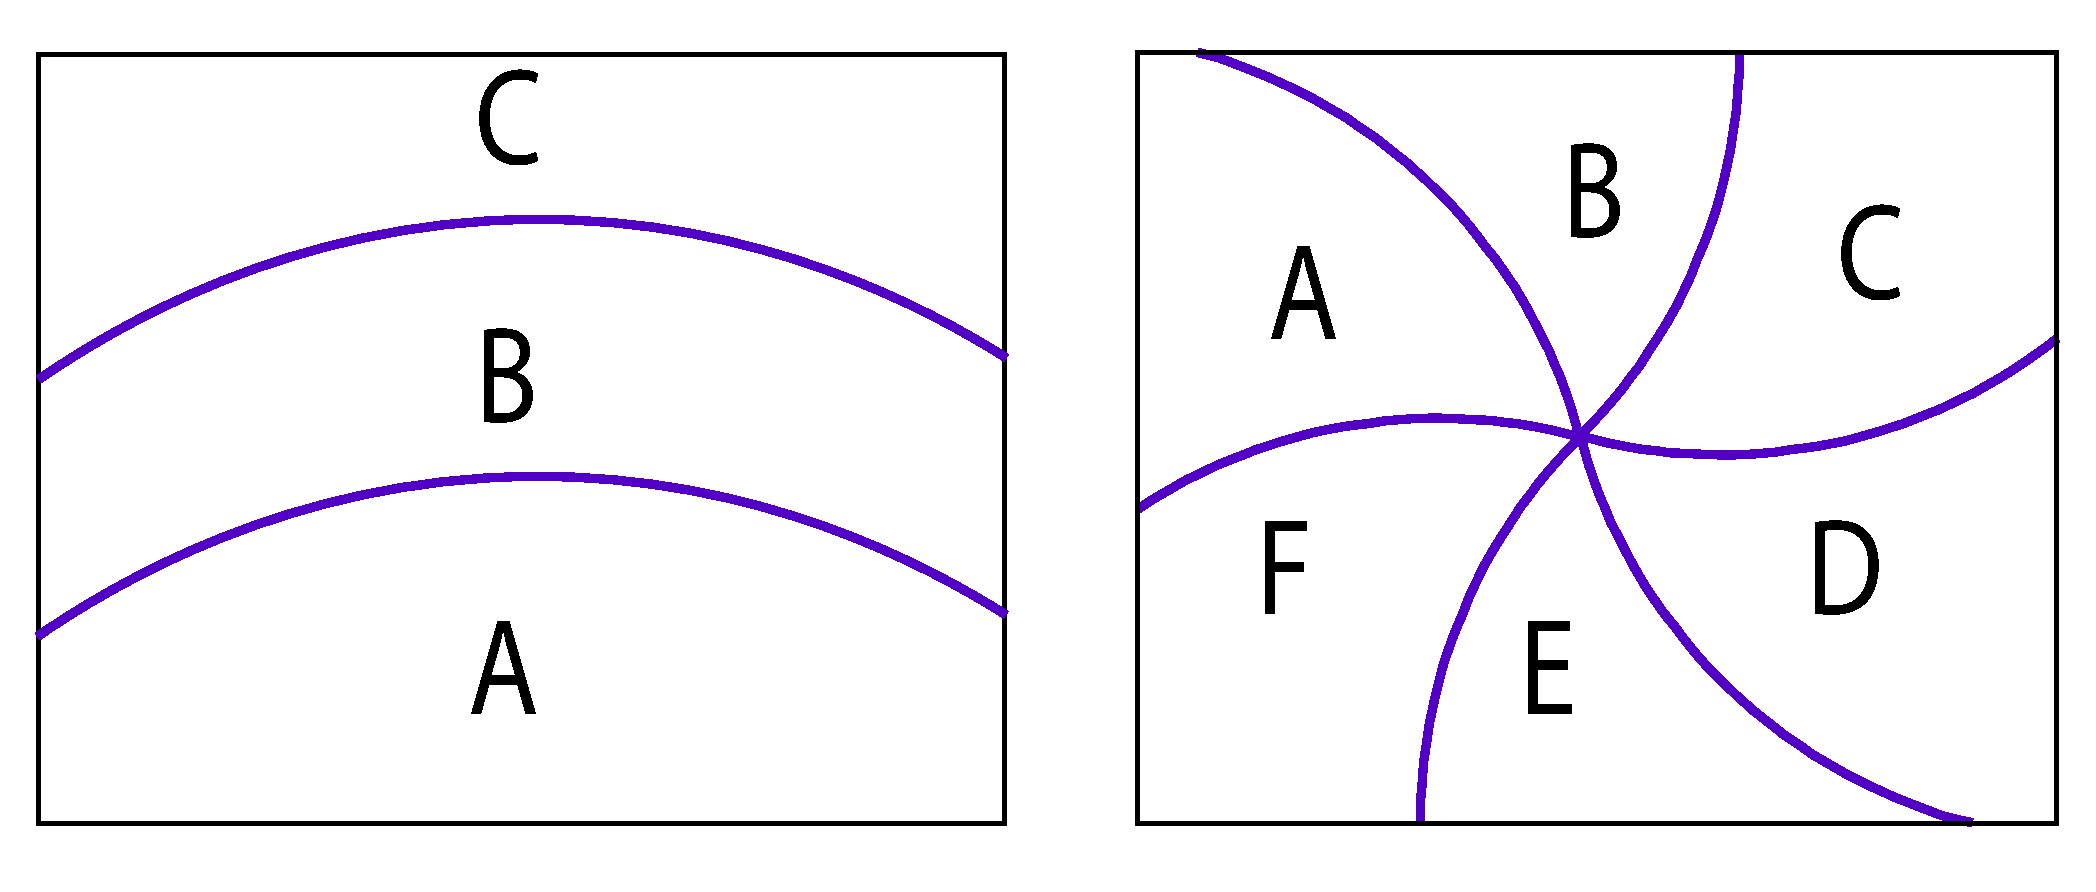
\includegraphics[width=\linewidth]{figures/multiple_crease_patterns}
	\caption{Propagation of constraints in crease patterns. Bottom row: Crease patterns. Top row: Curved folding of the crease patterns. Left and center columns: A deformation in the patch $P_1$ dictates most of the shape of the patch $P_2$, which in turn dictates most of the patch $P_3$. The propagation of deformation is generally global, and depends on the directions of the rulings. In these cases one can choose a mountain/valley assignment for one fold, which already determines the M/V assignment of the next fold (left: valley-mountain, center: valley-valley). Right column: In more complicated crease patterns, for instance those with a vertex, the process is more involved, as there are also some compatibility conditions the patches must satisfy. }
	\label{fig:multiple_crease_patterns}
\end{figure}

Generally speaking, one may be able to choose between four different configurations of the surface at one crease, but this choice already fixes the patch shape for nearby creases. The combinatorial degrees of freedom that remain are whether each crease is folded or not (see \figref{fig:folded_and_not_folded}). The difficulty in modeling folding of a planar surface stems from the fact that these combinatorial choices often need to be enforced at the beginning of the folding process, as explained by the following theorem.% combinatorial degree of freedom is often only available at the start of a deformation of a flat surface, as detailed in the following lemma:

\begin{theorem}\label{Thm:curved_folding_open_condition}
Let $S(t)$ be a curved folding flow and let $p(t_k)$ be a point on a curved crease of $S(t)$ lying on two patches $S_1(t),S_2(t)$ at a given time in the flow, $t=t_k$. If $p(t_k)$ is not a planar point on $S_1(t_k)$ (or equivalently on $S_2(t_k)$), then there exists an $\epsilon > 0$ such that one of the following holds:
\begin{enumerate}
	\item $\ S(t)$ is folded at $p(t)$ for every $t \in (t_k-\epsilon, \ t_k+\epsilon)$;
	\item $\ S(t)$ is \emph{not} folded at $p(t)$ for every $t \in (t_k-\epsilon, \ t_k+\epsilon)$.
\end{enumerate}
\end{theorem}
\begin{proof}
Let $\kappa(p(t))$ be the crease curvature at the point $p(t)$, and let $\kappa_g(p(t)) = \kappa(p(t))\cos\frac{\theta(p(t))}{2}$ be the crease's flattened (geodesic) curvature. If $\theta(p(t)) \neq 0$, the claim follows from the discontinuity of the two tangent planes at $p(t)$: a folding corresponds to a different choice of the tangent planes, forming an angle of $\theta(p(t))$ with each other, and any small continuous deformation cannot move from a folded to a non-folded configuration or vice-versa. Finally, the non-planarity of $p(t_k)$ implies $\theta(p(t_k)) \neq 0$, since $\theta(p(t_k)) = 0$ would mean that the normal curvature of the crease curve is $0$, and therefore the tangent of the crease curve is parallel to the ruling direction.
% (see inset). 
But by Lemma 12 and Corollary 16 in \cite{demaine_lens} this implies that the curve has a kink at  $p(t_k)$, contradicting the fact that $S(t)$ is $C^2$ when restricted to the patches $S_1(t), S_2(t)$.
\end{proof}
%\setlength{\columnsep}{8pt}%
%\begin{wrapfigure}{r}{0.3\linewidth}
%  \centering
%  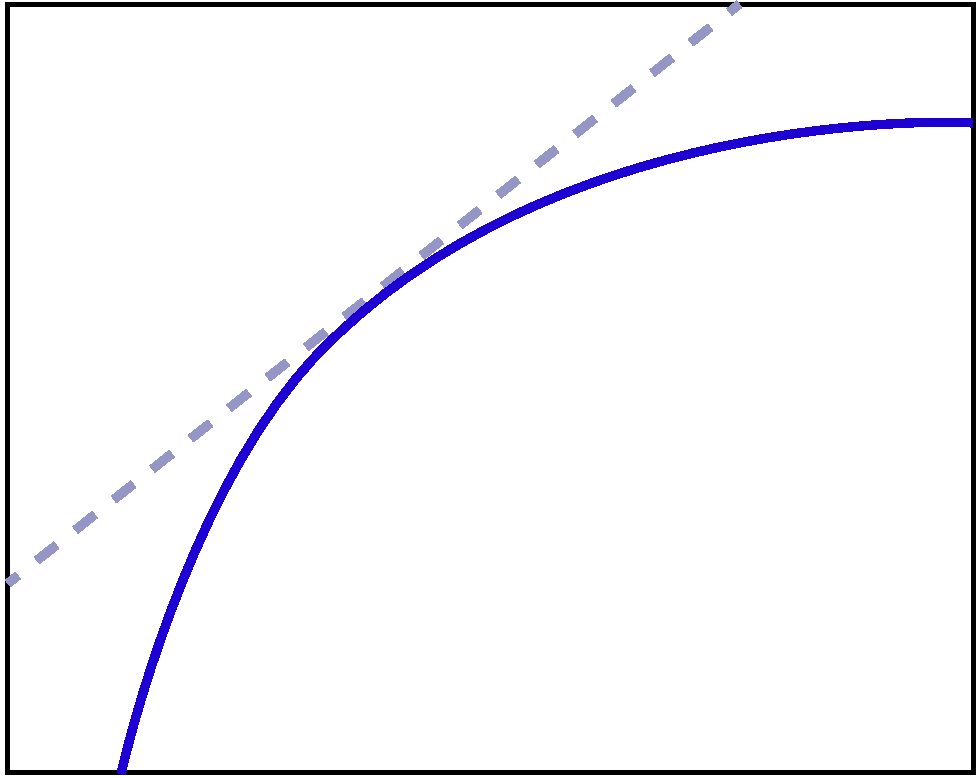
\includegraphics[width=\linewidth]{figures/ruling_tangent_to_a_curved_fold}
%%  \caption{\label{fig:cone_from_curve} A local representation of a developable surface through a curvature line curve $\gamma(s)$, and orthogonal rulings emanating from it.}
%\end{wrapfigure}

Therefore it is impossible to fold a crease point that is non-planar. For a non-planar point that is not folded, any small deformation keeps it that way. Folding can only happen after flattening the point, and if the surface is already folded, any small deformation keeps it folded. Thus, the decision whether to fold or not can only be done when the crease points are planar, and no extra care needs be taken if the crease is already folded. With this in mind, we note the following observation.

\begin{theorem}\label{Thm:supporting_plane}
A non-planar curved crease point $p$ on a curved folded surface $S$ is folded if and only if the osculating plane of the crease curve at $p$ is locally a supporting plane for the patches $S_1,S_2$ intersecting at $p$.
\end{theorem}
\setlength{\columnsep}{8pt}%
\begin{wrapfigure}{r}{0.2\linewidth}
  \centering
  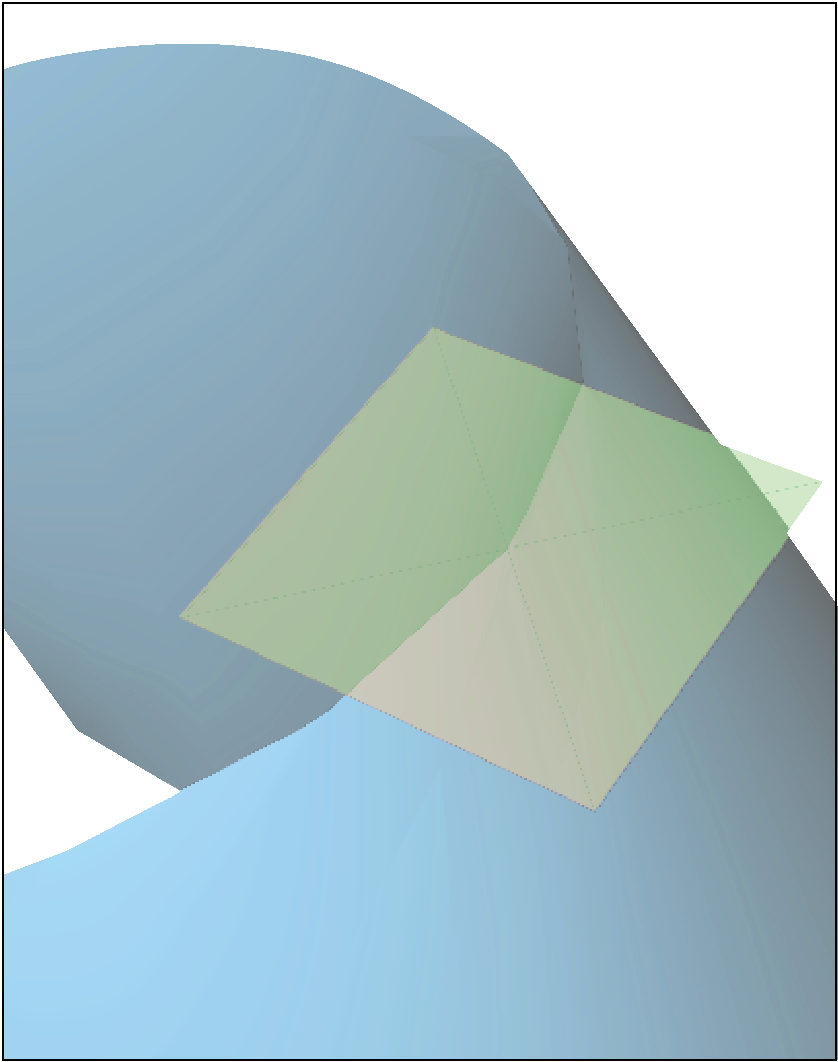
\includegraphics[width=\linewidth]{figures/plane_side.pdf}
\end{wrapfigure}
This follows directly from the fact that the tangent planes on both sides of a crease curve coincide if the surface is smooth there, but along a folded crease they are reflections of one another through the crease curve's osculating plane. Planar crease points along a curved crease, while not folded, still satisfy this constraint, since around these points the tangent planes are exactly the same as the osculating plane of the curve, though even the slightest surface deformation might change that. 

\subsection{Discretization}
We saw that folding happens exactly when both sides of the surface around a crease are in the same half-space of the osculating plane of the crease curve. We discretize this condition by constraining the tangents of the discrete parametric (grid) lines of the two DOG patches to be on the same side of the crease curve's discrete osculating plane. See \figref{fig:osc_plane_discretization} for the notation. The DOG edges intersecting the crease can be considered as discrete surface tangents originating at the crease points. In the notation of \figref{fig:osc_plane_discretization}, each of the two patches has its own duplicate of the edge ($e_1$ or $e_2$) intersecting the crease curve. In the starting, flat configuration the two edges coincide, but a folding movement creates a discontinuity between them. We denote the discrete surface tangents on both sides of the crease curve as $t_1 = \frac{e_1}{\|e_1\|}, t_2 = \frac{e_2}{\|e_2\|}$. The binormal of the crease curve, i.e., the normal of its osculating plane, is $B = \frac{e_f \times e_b}{\|e_f \times e_b\|}$, noting that $e_f,e_b$ always coincide for both patches.

\begin{figure} [t]
	\centering
	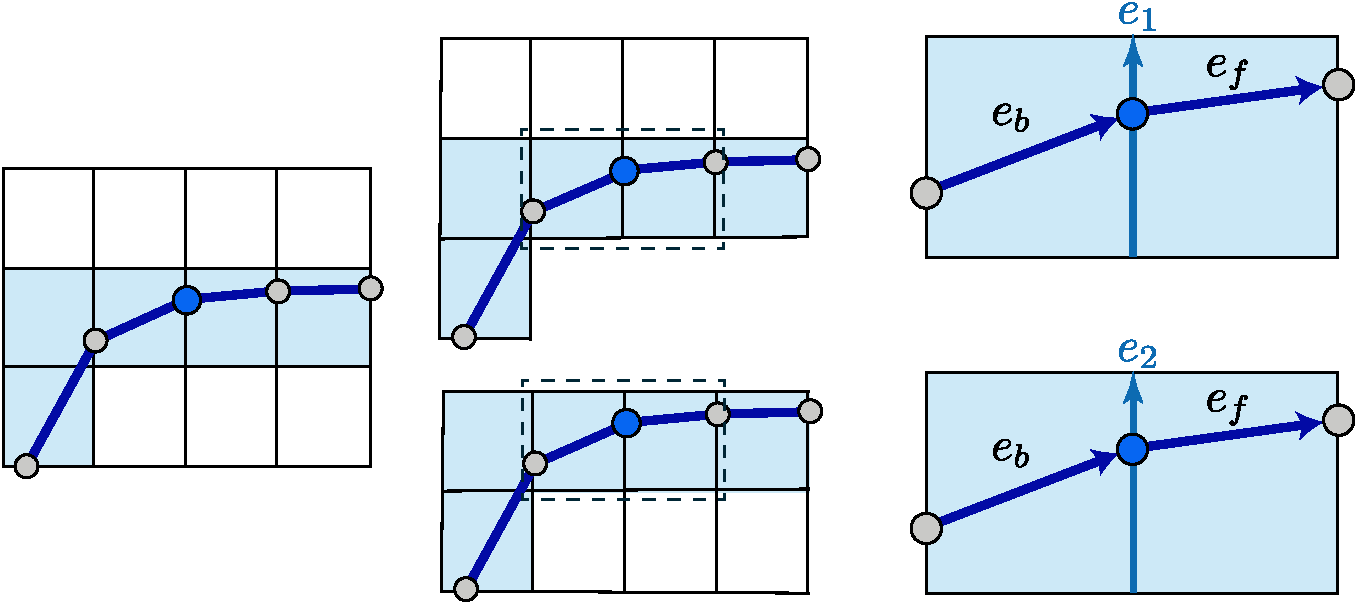
\includegraphics[width=\linewidth]{figures/osc_plane_discretization}
	\caption{Notation for edges in a discrete crease pattern. Left: a flat DOG with a discrete crease curve. Center: Following \cite{rabi2018shape}, we represent creases by duplicating the quads that contain the crease curve, which results in different connected components, or patches. The positions of the vertices on the curve, i.e., its intersection points with the grid edges, are constrained to match on both patches. Right: Notation for a duplicated grid edge ($e_1, e_2$) intersecting the crease curve at the blue point, and the two crease edges $e_f,e_b$. }
	\label{fig:osc_plane_discretization}
\end{figure}

The supporting plane constraint can be written as
\begin{equation} \label{eq:folding_const_normalized} 
\text{sgn}(\langle t_1,B\rangle) +  {sgn}(\langle t_2,B\rangle) = 0
\end{equation}
with 
\begin{equation} \label{eq:sign}
\text{sgn}(x) = \left\{
     \begin{array}{@{}r@{\thinspace}l}
       -1  &: \text{if } x < 0, \\
       0 &: \text{if } x = 0, \\
       1 &: \text{if } x > 0. \\
     \end{array}
   \right.
\end{equation}
%
Constraint \eqref{eq:folding_const_normalized} can be simplified by replacing $B$ with the cross product $e_f \times e_b$. Furthermore, if one assumes an isometric deformation, it is possible to replace $t_1,t_2$ by the non-normalized edges $e_1,e_2$, arriving at:
\begin{equation} \label{eq:folding_const}
\text{sgn}(\langle e_1,e_f \times e_b \rangle) +  {sgn}(\langle e_2,e_f \times e_b\rangle) = 0.
\end{equation}
In \secref{sec:implementation} we show how to plug this constraint into an optimization framework to model folding and bending of curved folded DOGs (see \figref{fig:folded_and_not_folded}).

\subsection{Discussion}
There are multiple equivalent characterizations for a folded crease over a curved folded surface. We now point out some key properties of our chosen discretization \eqref{eq:folding_const_normalized} and briefly discuss how these properties are \newt{not satisfied} by other possible constraint choices.

\paragraph{Suitable for homotopy based optimization methods} 
Our constraint is satisfied on a flat mesh. In this sense we consider a point along a curve with zero normal curvature as both folded and not folded.
 
\paragraph{Minimal and generally non-intrusive} 
Once a curved crease on a piecewise DOG is folded, one no longer needs to take explicit care for it to stay folded. The effect of \equref{eq:folding_const} on an already folded surface is null. The tangent discontinuity caused by the folding implies that a folded crease remains folded under local deformations, and in order for it to become unfolded, one needs to first flatten it, as is the case for a piecewise smooth curved folded surface. We also capture the converse: a discrete curved crease can only be folded when starting from a planar point (\theoremref{Thm:curved_folding_open_condition}). \\

An alternative constraint for folding could be e.g.\ enforcing discontinuities along the tangents $t_1,t_2$, but this results in losing the feasibility of the flat models. Moreover, in the discrete case a minor discontinuity can still arise even though there is no fold, i.e., where \equref{eq:folding_const_normalized} is not satisfied, thus numerically giving the impression of a fold when visually there is none. Another option is to define folded configurations as those satisfying a similar but simpler smooth constraint:
%
\begin{equation} \label{eq:folding_const_smooth} 
\langle t_1,B\rangle + \langle t_2,B\rangle = 0.
\end{equation}
%
This condition is satisfied exactly in flat models and in any piecewise smooth curved folded surface, since tangent planes along a folded creased curve are reflections of each other w.r.t.\ the osculating plane of the crease curve. However, this condition is not satisfied \emph{exactly} on every folded piecewise DOG (as evident by all models in this paper). An exception to this is the class of curved creases with zero torsion, in which case the folds are simply formed as a global plane reflection \cite{Mitani_ref}. Therefore, enforcing constraint \eqref{eq:folding_const_smooth} as a hard constraint is too restrictive in practice, while enforcing it softly creates a condition that, unlike the smooth case, does not vanish once a crease is folded and hence is not minimal in our sense.


\section{Folding angles and mountain-valley assignments} \label{sec:folding_angles_mountain_valley}

In this section we propose tools to constrain the folding angles and their direction (mountain or valley) during deformation, in order to provide designers with additional expressive and intuitive control. We first show how to constrain folding angles, i.e., the angles between the tangent planes around a crease. We implement this by constraining DOG tangent angles, resulting in a simple quadratic constraint. We then devise a tool to differentiate between mountain and valley folds. Our derivations work for both curved and straight origami creases.

\begin{figure} [b]
	\centering
	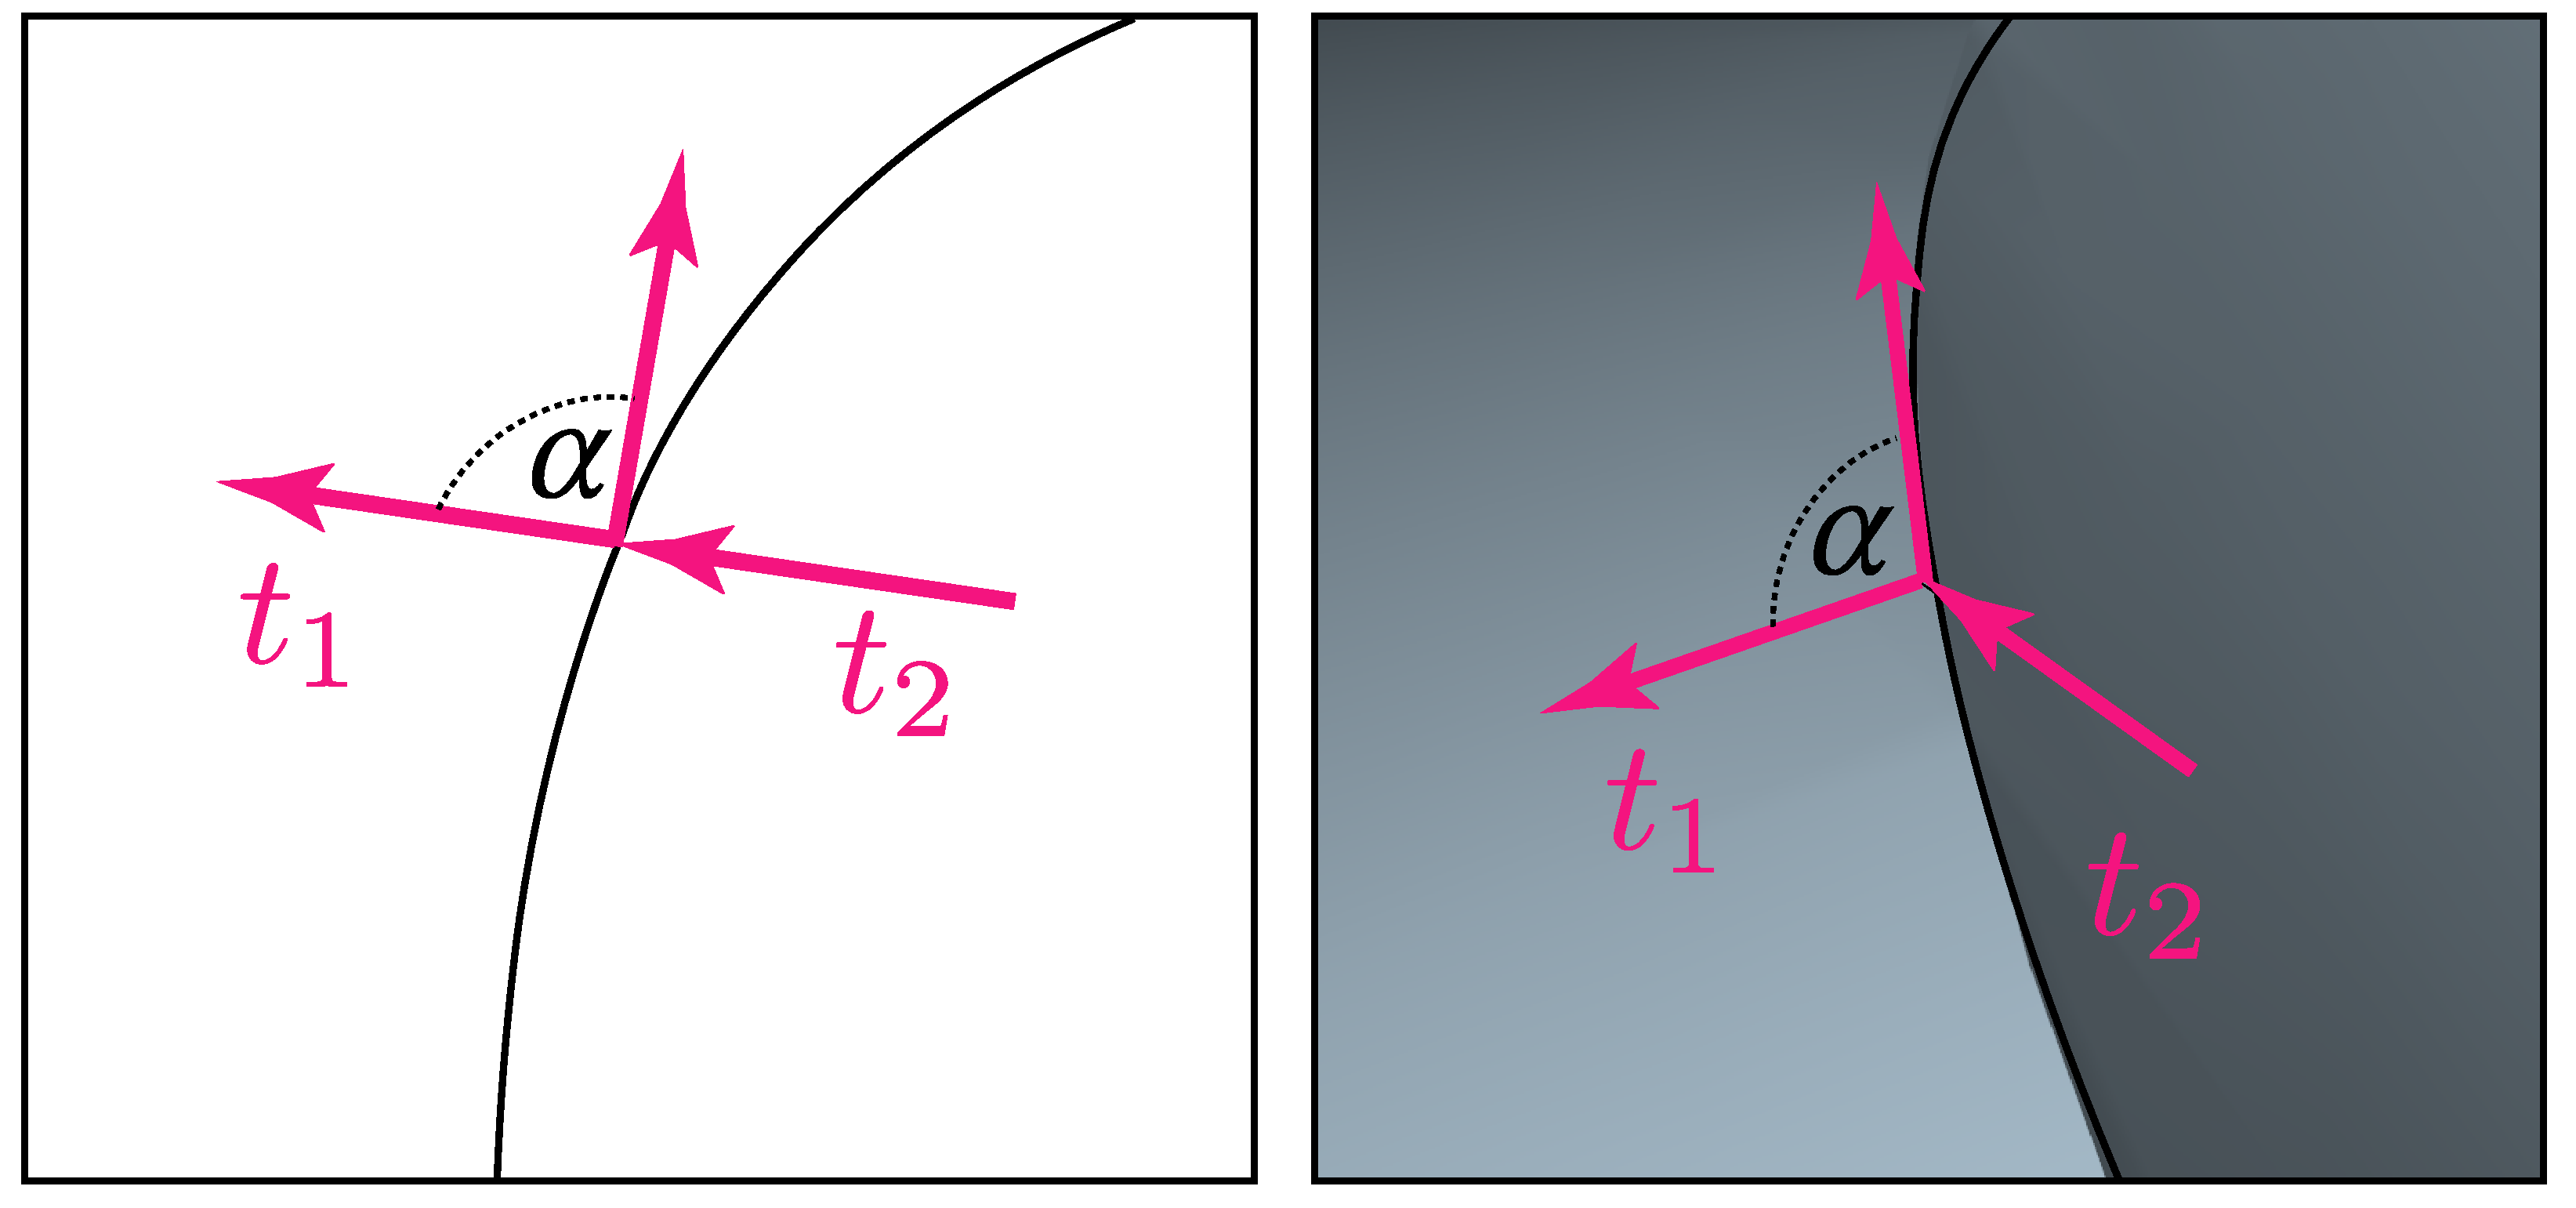
\includegraphics[width=0.7\linewidth]{figures/fold_angles_smooth}
	\caption{Left: A flattened configuration of a crease curve and its tangent $t$, forming an angle $\alpha$ with surface tangents $t_1,t_2$, which are equal in this flat state ($t_1=t_2$). Right: A folded isometric configuration with a tangent discontinuity  $t_1 \neq t_2$. \lemmaref{lem:tangents_dihedral} shows the connection between the angle $\alpha$ and the folding angle $\theta$ in the smooth case, stating that $\langle t_1, t_2 \rangle = \cos^2\!\alpha + \sin^2\!\alpha \cos\theta$.}
	\label{fig:fold_angles_smooth}
\end{figure}

\subsection{Folding angle} \label{sec:folding_angle}

A folding deformation can be seen as a rotation of the surface patches' tangent planes hinged on the tangent of the crease curve. The tangent of a straight fold is constant, and so is the folding angle, while on a curved crease, the tangent varies and often the folding angles change along the crease. In both cases, if the folding angle at a given point is $\theta$, then the surface tangent vectors on both sides of the crease that are orthogonal to the crease tangent form an angle of $\theta$, while the surface tangent vectors that are parallel to the crease remain parallel to each other. The following lemma shows the relation between the angle formed by surface tangent vectors that are equal in the flattened configuration and the folding angle (see \figref{fig:fold_angles_smooth}): 
\begin{lemma}  \label{lem:tangents_dihedral}
	Let $t_1,t_2$ be surface tangent vectors on two sides of a crease curve at a given point $p$ that are equal to each other in the isometrically flattened state of the developable surface. Let $t$ be the crease curve tangent at $p$. Assuming the surface went through a curved folding isometric deformation and the folding angle at crease point $p$  is $\theta$, the surface tangent vectors satisfy:
	\begin{equation} \label{eq:tangents_dihedral}
	\langle t_1, t_2 \rangle = \cos^2\!\alpha + \sin^2\!\alpha \cos\theta, \end{equation}
	%4*cos(alpha/2)/(norm(e1)+norm(e2))
	where $\alpha$ is the angle between $t$ and $t_1$. Note that this angle is preserved under isometry.
\end{lemma}
\begin{proof}{We denote by $t,n,b$ the vectors of the Frenet frame of the curved crease at $p$. We wish to express the surface tangent vectors $t_1, t_2$ in the local coordinates of this Frenet frame. In the flat isometric configuration, $t_1, t_2$ coincide and can be written as $\cos(\alpha)t + \sin(\alpha)n$. A folding angle of $\theta$ means that relative to the Frenet frame of the curve, the surface tangent on one side of the curve was rotated by angle $\frac{\theta}{2}$ about the crease curve tangent $t$, and the surface tangent on the other side by  $-\frac{\theta}{2}$. 
		%
		Thus w.l.o.g.\ 
		\begin{align*}
		\textstyle t_1 = \cos(\alpha)t + \sin(\alpha)\left(\cos\left(\frac{\theta}{2}\right)n + \sin\left(\frac{\theta}{2}\right)b\right),\\
		\textstyle t_2 = \cos(\alpha)t + \sin(\alpha)\left(\cos\left(\frac{\theta}{2}\right)n - \sin\left(\frac{\theta}{2}\right)b\right). 
		\end{align*}
		%
		The proof is concluded by computing $\langle t_1,t_2 \rangle$ and plugging in the trigonometric identity $\cos\theta = \cos^2{\frac{\theta}{2}}-\sin^2\frac{\theta}{2}$.}\end{proof}



We discretize \lemmaref{lem:tangents_dihedral} by looking at angles between edges of the DOG emanating from crease points (see \figref{fig:fold_angle_and_tangent_angles}). Using the notation of \figref{fig:fold_angle_and_tangent_angles}, we discretize the tangent of the crease curve at a given point by looking at the incident edge vectors $e_f, e_b$: 
\begin{equation} \label{eq:crease_tangent}
t = \frac{\|e_b\|e_f + \|e_f\|e_b}{\left\|\|e_b\|e_f + \|e_f\|e_b\right\|}.
\end{equation}
If the two edge vectors $e_b, e_f$ are not collinear, $t$ as above is the tangent at the point to the unique circle passing through the point and its two neighbors. 

Under an isometric deformation, $t_1,t_2$ are linear in the vertex positions, $\alpha$ is constant and  \equref{eq:tangents_dihedral} is quadratic.

\begin{figure} [t]
	\centering
	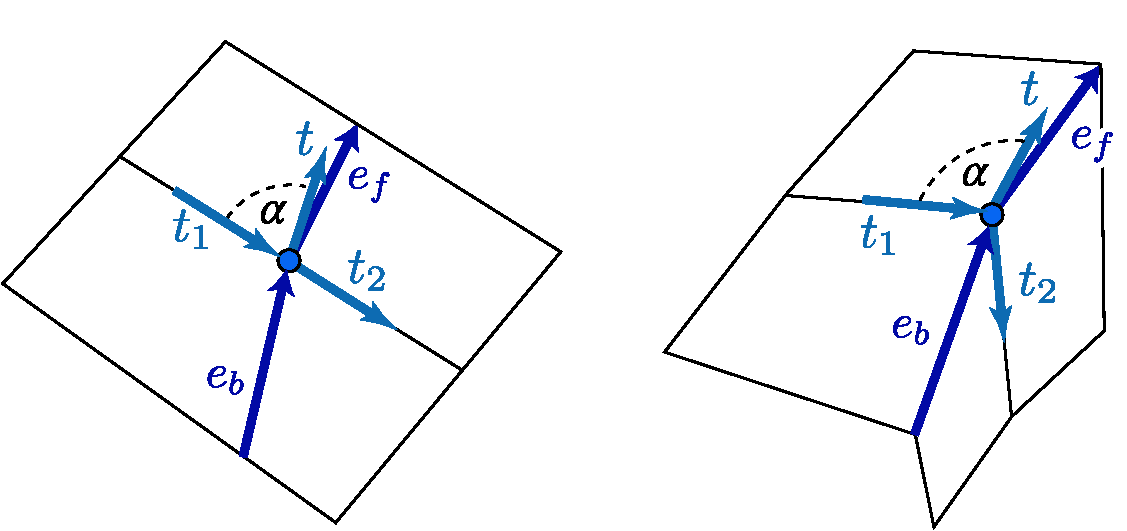
\includegraphics[width=0.8\linewidth]{figures/fold_angle_and_tangent_angles}
	\caption{Discretizing \lemmaref{lem:tangents_dihedral} (see \figref{fig:fold_angles_smooth}) at a crease point by using the normalized DOG edges emanating from the crease point as surface tangents.}
	\label{fig:fold_angle_and_tangent_angles}
\end{figure}

\subsection{Mountain/valley assignments} \label{sec:MV_assignments}
As mentioned in \secref{sec:smooth-combinatorial}, there are a few combinatorial degrees of freedom in choosing the type of fold, i.e., the choice of surfaces on each side of the curve (\figref{fig:folding_combinatorics}). We follow \cite{demaine_lens} to distinguish between the two types of folded configurations in \figref{fig:folding_combinatorics} by calling one choice a \emph{mountain fold} and the other a \emph{valley fold}. We would like to emphasize that for straight folds, this degree of freedom always exists, but on curved creases it often does not. In fact, in many crease patterns it is often only possible to choose one mountain/valley (M/V) assignment, and the remaining assignments are determined by the propagation of the rulings, leaving only the combinatorial degrees of freedom of whether a crease is folded or not, embodied by \equref{eq:folding_const_normalized}. 
%For instance, in \cite{demaine_lens} the authors prove how segments on the convex side of a crease bend mountain/valley the same as the crease, while segments on the concave side of a crease bend mountain/valley opposite from the crease. This can be seen in \figref{fig:multiple_crease_patterns}, where the left crease pattern has a mountain and valley fold while the center one has only valleys.
 We distinguish M/V folds by looking at whether a tangent of one surface patch is above or below the tangent plane of the second surface patch at the crease point, for a consistent choice of orientation. This can be achieved by the following constraint:
\begin{equation} \label{eq:mountain_valley_ineq}
\langle t_1, t \times t_2 \rangle \leq 0,
\end{equation}
where $t$ is the tangent of the oriented crease curve and $t \times t_2$ is the normal of the tangent plane of the second surface patch (the one that has $t_2$ as a tangent vector). The orientation of $t$ determines whether a mountain or a valley fold is chosen. By the cyclic property of the triple product, the left hand side of \equref{eq:mountain_valley_ineq} is also equal to $\langle t_2, t_1 \times t \rangle$.
As we are only interested in the sign of the left side of \eqref{eq:mountain_valley_ineq}, we can replace $t$ with the simpler $t^* = \|e_b\|e_f + \|e_f\|e_b$, which is linear under isometry.
 
To simplify notation for \secref{sec:implementation}, we reformulate our mountain/valley constraint with an equality by using the Heaviside step function:
\begin{equation} \label{eq:heaviside}
\text{H}(x) = \left\{
     \begin{array}{@{}l@{\thinspace}l}
       0  &: \text{if } x \leq 0, \\
       1 &: \text{if } x > 0, \\
     \end{array}
   \right.
\end{equation}
and write the mountain/valley condition as:
\begin{equation} \label{eq:mountain_valley}
H(\langle t_1, t^* \times t_2 \rangle) = 0.
\end{equation}
% !TEX root =  CurvedFoldedDogs.tex

\section{Optimization} \label{sec:implementation}
We employ \theoremref{Thm:supporting_plane} and its discretization in \equref{eq:folding_const} in a simple algorithm to enforce folding along crease curves while deforming piecewise DOGs. The algorithm aims to minimize an objective function while keeping the DOG constraints and ensuring the formation of folds along all crease curves.

\subsection{Problem setup}
We model our curved folded surfaces as a quad mesh, with a separate connected component for each patch. We denote the set of $n$ mesh vertices in $\R^3$ by $V$, the vertex positions (variables) by $\x \in \R^{3n}$, and the quad mesh faces by $F$. Each connected component is a DOG, i.e., it has the connectivity of a subset of $\Z^2$ and satisfies the DOG angle constraints \cite{rabi18}, which we denote as $\phi_{d_i}(\x) = 0, 1 \leq i \leq m$.

We are interested in deformations that fold the surface along all crease curves in a given crease pattern using \theoremref{Thm:supporting_plane} and enforcing \equref{eq:folding_const}. We enforce these constraints on all crease points, which are points on crease curves that are not crease vertices, with the exception of crease points that have the following degeneracies on the flattened mesh (see \figref{fig:fold_const_degeneracies}):
\begin{enumerate}
	\item degenerate osculating plane: crease points with a curvature smaller than a threshold $\kappa_\eps$; \label{item:deg_osc}
	\item degenerate edge: crease points on an edge, splitting it into two parts where one is shorter than $\eps_{r}$\% of the other; \label{item:deg_edge}
	\item degenerate angle with the intersecting DOG tangent: crease points where the tangent directions $t_1,t_2$ form an angle with one of the edges $e_f,e_b$ that is smaller than $\eps_\alpha$. \label{item:deg_tan_angle}
\end{enumerate}
We use the constants $\kappa_\epsilon=\text{1e-5}, \eps_r=5\%, \eps_\alpha=3^{\circ}$. We denote the folding constraints by $\phi_{f_j}(\x) = 0, 1 \leq f_j \leq n_f$.

\begin{figure} [h]
	\centering
	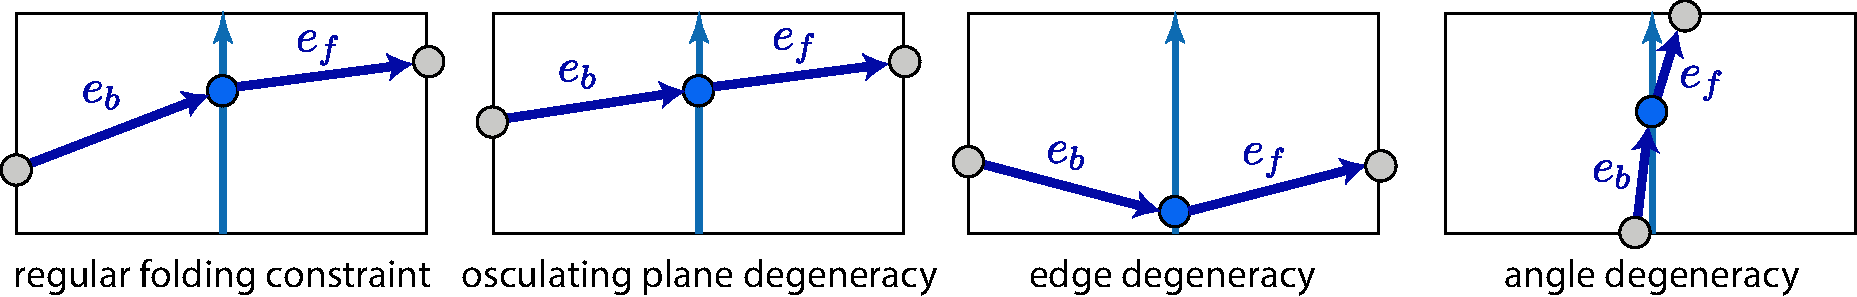
\includegraphics[width=\linewidth]{figures/fold_const_degeneracies}
	\caption{A folding edge constraint defined on a blue crease point splitting the blue edge and degenerate cases where we do not enforce the constraint. From left to right: A regular folding edge constraint, instabilities in the osculating plane's normal as $\frac{e_b \times e_f}{\|e_b \times e_f\|}$ caused by $e_b,e_f$ being almost collinear, degenerate edges as one part of the edge split by the blue crease point is comparably very short, and lastly a very small angle between $e_b$ and the DOG edge crossing the blue point. An angle degeneracy often occurs before or after an edge degeneracy.}
	\label{fig:fold_const_degeneracies}
\end{figure}

The problems we solve in this paper can be written in the form:
\begin{equation} \label{eq:const_opt}
\begin{aligned}
& \argmin_x f(x) \\
& \textrm{subject to} \\
& \phi_{d_i}(\x) = 0, \ \  i = 1, \ldots, m, \\
& \phi_{f_j}(\x) = 0, \ \  j = 1, \ldots, n_f, \\ 
\end{aligned}
\end{equation}
where $f$ is an objective function composed of a weighted sum of a bending objective, isometry objective, positional constraints and other terms as specified in \secref{sec:dog_obj}.

\subsection{Folding constraints}
Motivated by the fact that in the smooth case, one cannot move from a folded to a non-folded configuration around a non-planar point, we strive to always satisfy $\phi_{f_j}(x) = 0$ exactly. The common starting point of a flat surface is an interesting case, as it is a bifurcation point between surfaces satisfying \theoremref{Thm:supporting_plane} and those that do not, which also holds for the discretization \equref{eq:folding_const_normalized}. To that end, we solve our problem with an iterative sequential quadratic programming (SQP) solver with a line search, complemented with two simple strategies to handle the folding constraints $\phi_{f_i}(\x)$:
\begin{enumerate}
	\item a penalty term \cite{nocedal} punishing  deviation from the constraints; \label{opt:penalty}
	\item a line search method that backtracks if the resulting mesh does not exactly satisfy $\phi_{f_j}(\x) = 0, i = 1,...,n_f$.
\end{enumerate}
Since the functions $\text{sgn}(x),H(x)$ involved in the constraints $\phi_{d_i}(\x)$ are not $C^1$, we replace them by the approximations:
%
\begin{align} 
\begin{split}\label{eq:const_inner}
&\text{sgn}(x) \approx \tanh(hx) \\
&H(x) \approx  \left\{\begin{array}{@{}l@{\thinspace}l}
0  &: \text{if } x \leq 0, \\
\frac{x^2}{x^2+\delta} &: \text{if } x = 0, \delta > 0 \\
\end{array}\right.
\end{split}
\end{align}
using the fixed parameters $h=1000,\delta = \text{1e-5}$. Our approximation for $H(x)$ is taken from \cite{l0_approximation,autocuts}.  The use in a homotopy based optimization necessitates an approximation for $H(x)$ that vanishes on a flat mesh, and therefore we do not use the common approximation for the Heaviside function $H(x) \approx \hat{H}(x) =  \frac{1+\tanh(hx)}{2}$ because $\hat H(0) = \frac{1}{2}$.

We refer to the approximated constraints as $\phi^*_{f_j}(\x)$ and replace the optimization problem \eqref{eq:const_opt} with the following problem:
\begin{equation} \label{eq:const_opt_penalty}
\begin{aligned}
& \argmin_x f(x) + \omega \sum \|\phi^*_{f_j}(\x)\|_2^2 \\
& \textrm{subject to} \\
& \phi_{d_i}(\x) = 0, \ \  i = 1, \ldots, m. \\ 
\end{aligned}
\end{equation}
Here, $\omega > 0$ is a metaparameter initialized as $\omega_0 = 1$, which doubles its value if the line search cannot find a point satisfying the supporting plane conditions exactly. In practice, the penalty term only affects points that are very close to being planar, while approaching zero very quickly around already folded points.

\subsection{Equality constrained SQP}
For ease of notation, we use the following to refer to the objective of \equref{eq:const_opt_penalty}:
\begin{equation}
f_\omega(\x) = f(x) + \omega \sum \|\phi^*_{f_j}(\x)\|_2^2.
\end{equation}
We minimize \eqref{eq:const_opt_penalty} using SQP with a line search \cite{nocedal}. Given a set of variables at a given iteration $x^k$ and current values of Lagrange multipliers $\lambda^k$, a line search equality constrained SQP algorithm iteratively finds the next direction for a line search of \equref{eq:const_opt_penalty}, by which it sets the next variables $x^{k+1}$ by solving a KKT system of the form:
%
\begin{equation} \label{eq:KKT_eps}
\begin{aligned}
&{K} \begin{pmatrix} d^{k+1} \\ \lambda^{k+1} \end{pmatrix}=\mathbf{b}, \ \text{where} \\
&{K}=\begin{pmatrix}
{\Delta^2_{xx}\mathcal{L}(x^k,\lambda^k)} & {J^\tr}(\x^k)\\
{J(\x^k)} &  0 \\
\end{pmatrix}, \ \ 
\mathbf{b}=\begin{pmatrix}
{\nabla f_\omega(x^k)} \\ 
-\phi_{d_i}(x^k)\\
\end{pmatrix},
\end{aligned}
\end{equation}
%
where $J(\x)$ is the Jacobian of the equality constraints in \equref{eq:const_opt_penalty}, $\Delta^2_{xx}\mathcal{L}(x,\lambda) = H_{f_\omega}(x)+\sum\lambda_i^{k} \nabla \phi_{d_i}(x)$ is the Lagrangian of the problem and $H_{f_\omega}(\x)$ is the Hessian of $f_\omega(\x)$.

Following \cite{rabi2018shape}, we use a minimally modified Jacobian $J^*(x)$ to deal with singularities in DOGs. We also replace the Hessian of the objective $H_{f_\omega}(\x)$ by a convex approximation, which we denote by $H^*_{f_\omega}(\x)$, as detailed in \secref{sec:dog_obj}, and thus replace the system \eqref{eq:KKT_eps} by:
%
\begin{align} 
\label{eq:linear_system}
&{K} \begin{pmatrix} d^{k+1} \\ \lambda^{k+1} \end{pmatrix}=\mathbf{b}, \ \text{where} \\
\nonumber
&{K}=\begin{pmatrix}
{ H^*_{f_\omega}(\x^k)+\sum\lambda_i^{k} \nabla \phi_{d_i}(\x^k)} & {J^{*^\tr}(\x^k)}\\
{J^*(\x^k)} &  0 \\
\end{pmatrix}, \ \ 
\mathbf{b}=\begin{pmatrix}
{\nabla f_\omega(x^k)} \\ 
-\phi_{d_i}(x^k)\\
\end{pmatrix}.
\end{align}

We note that in \cite{rabi2018shape} the authors discretize Laplacian metric flows by solving a similar system with a Laplacian instead of the objective's Lagrangian. However, we found that replacing the Laplacian by the Lagrangian followed by convexifying the Hessian performs significantly better, especially on larger models. As common in SQP algorithms, we use a merit function to guide our line search, defined as a combination of the objective and the constraints. The line search chooses step sizes that reduce the objective and keep the DOG angle constraints numerically feasible, while backtracking if a point does not satisfy the folding constraints exactly.

This removes the need for the slower LBFGS constraints' projection used by \cite{rabi18,rabi2018shape}. We use the $L_2$ merit function \cite{nocedal}:
\begin{equation}
\psi(\x;\mu) = f_\omega(\x)+\mu\sum\|\phi_{d_i}(x)\|_2,
\end{equation}
where we update the parameter $\mu^k$ at each iteration using the absolute values of the Lagrange multipliers \cite{nocedal}:
\begin{equation}
\mu^k = \max\{c_\mu \cdot \max\{|{\lambda_i^k}|\},\ \mu_0\},
\end{equation}
with $c_\mu = 1.1$ and $\mu_0 = 0.05$.

\subsection{Objectives and constraints} \label{sec:dog_obj}
Our objective $f$ is composed of a weighted sum of various functions measuring bending, stretch, positional constraints and dihedral angles.
We use an integrated squared mean curvature bending objective taken from \cite{rabi2018shape}, and we exploit the fact that it is quadratic and convex under isometric deformations (\cite{quadratic_bending}):
\begin{equation}
f_\text{H}(\x) = 0.5\x^t(L^tM^{-1}L)\x,
\end{equation}
where $L$ is the DOG Laplacian and $M$ is a diagonal mass matrix defined by the DOG vertex area \cite{rabi2018shape}.

 We employ \lemmaref{lem:tangents_dihedral} to constrain the folding angle at a given crease point using the constraint
\begin{equation}
\phi_{\text{d}_{c^i}}(\x) := \langle t_1^i, t_2^i \rangle - \cos^2(\alpha^i) - \sin^2(\alpha^i) \cos(\theta^i) = 0,
\end{equation}
where $c^i$ is the index of the crease point along the edge defined as a linear combination of two vertices, $t_1^i$, $t_2^i$, $\alpha^i$ are as defined in \secref{sec:folding_angle} and \figref{fig:fold_angle_and_tangent_angles}, and $\theta^i$ is the desired dihedral angle at the crease point $c^i$. Under isometry $t_1^i,t_2^i$ are linear in the net vertex locations, $\alpha^i$ is fixed, and the constraint is quadratic.

Let $e$ be an edge on the net mesh, $l_e$ its length and $l_e^0$ the length in the reference net mesh. We define the following quadratic isometry constraints:
\begin{equation}
\phi_\text{iso}(\x)_e := l_e^2 - {l_e^0}^2 = 0.
\end{equation}
We maintain continuity along the patches with a set of linear equality constraints on duplicated crease points \cite{rabi2018shape}, which we denote by $\phi_\text{cont}(\x) = 0$. Lastly, we allow the user to specify positional constraints on vertices or crease edge points, including constraints requiring two points to have the same coordinate (\MiR{point to teaser or sphere figure}, denoting this user defined set of constraints by $\phi_{\text{pos}}(\x) = 0$.
We enforce the dihedral, positional, isometry and patches continuity constraints in a soft manner by using a penalty on their squared deviation, denoted accordingly by $f_\text{D}(\x), f_\text{pos}(\x), f_\text{iso}(\x), f_\text{cont}(\x)$. These sum of squares objectives are not convex, and we replace their Hessian in our optimization with their Gauss-Newton's Hessian approximation. We do the same for $\sum \|\phi^*_{f_i}(\x)\|_2^2$. Isometry is enforced as a soft constraint $f_\text{iso}(\x)$, as advised by the degrees of freedom analysis in \cite{rabi18,rabi2018shape}, but we emphasize that all our results have an average relative edge stretch that is less than $0.003$, and a maximum stretch below $4$, where our surfaces are normalized to have an average edge length of $1$. As opposed to \cite{rabi2018shape}, we also encode  $\phi_\text{cont}(\x)$  as a soft constraint, as we have noticed a significant improvement in the quality and smoothness of crease patterns when these are enforced as a soft penalty with a large weight,
%\MiR{ok to say?, this is mostly important in the curved constrained case for interactivity, as if we run the interpolation much slower then we can still use hard constraints},  
and our results have an average continuity deviation of $0.0002$ and a maximum of $0.0035$. We note that the constrained shape space analysis in \cite{rabi2018shape} only concerns the DOG angle constraints, and complicated crease patterns give rise to a large set of additional linear constraints.
 
The objective we optimize is then:
\begin{equation} \label{eq:opt}
f(\x) = w_Hf_\text{H}+w_{pos}f_\text{pos}+w_Df_\text{D}+w_{iso}f_\text{iso}+w_{cont}f_\text{cont}
\end{equation}
Throughout the paper, unless stated otherwise, we use $w_H = 1$, $w_\text{pos}=5$,$w_D = 100$, $w_\text{iso}= \frac{20000}{\|E\|}$, $w_{cont} = 1e4$, where $\|E\|$ is the number of edges in the net mesh (i.e., for a mesh with $1000$ vertices $w_\text{iso}=20$). Our meshes are always scaled to have an average edge length of $1$ and therefore using a different resolution for the same geometry keeps our bending objective the same, but scales the isometric objective by the number of edges.
\section{Results} \label{sec:results}
\subsection{Editing system}
\begin{figure} [h]
	\centering
	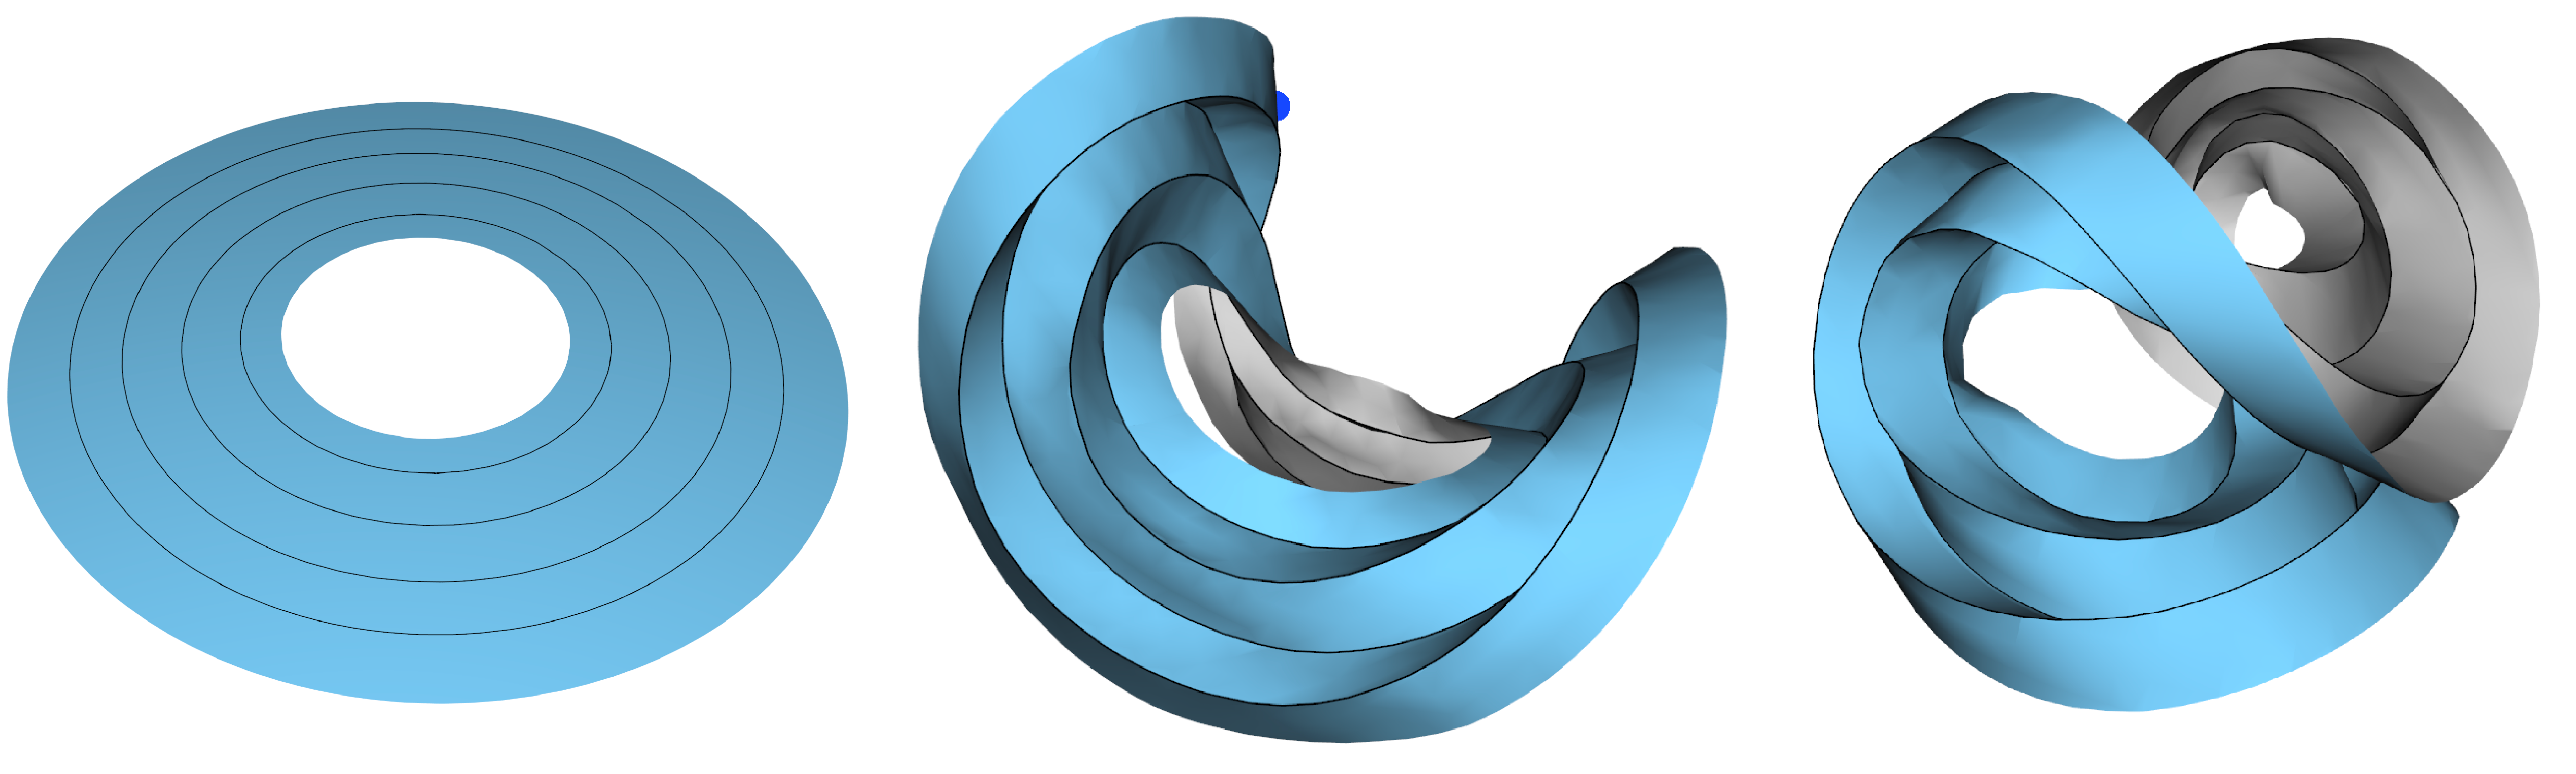
\includegraphics[width=\linewidth]{figures/annulus}
	\caption{\MiR{probably a temporary figure} }
	\label{fig:annulus}
\end{figure}
\subsection{Symmetry}
\subsection{Moving creases}
\section{Conclusions and future work}
This paper is a first step towards unhindered freeform modeling of curved folded surfaces. Basing our models on DOGs \cite{rabi18} allows us to capture the full set of curved folded deformations, and our discretization in \secref{sec:folding}, together with the folding algorithm in \secref{sec:implementation}, allows us to steer the modeled deformations towards those that simultaneously fold and bend crease curves. Our deformation algorithm is able to model bending and folding of complicated crease patterns by merely using positional constraints, making it highly suited for exploration of new curved folded surfaces. We supply further optional objectives to constrain dihedral angles and mountain/valley assignments in \secref{sec:folding_angles_mountain_valley}, providing designers additional expressiveness. 

Similar to other works on modeling DOGs \shortcite{rabi18,rabi2018shape}, the most obvious limitation of our algorithm is speed. Our optimization framework allows us to interactively model up to 2000 vertices. We leave scaling of the optimization to future work, possibly by using a multigrid solver on the DOG grids. In addition, we find that we lack tools and objectives to enforce symmetry of the designed shapes. In particular, we would like to look at folding of curved symmetric plane wallpapers and tessellations \cite{demaine_lens,mundilova2019mathematical}. We also do not take physical reality constraints into account, such as collisions, material thickness and elasticity properties, making the models created in our system not necessarily realizable. Incorporating our model into a physically accurate design system could potentially alleviate this limitation. Finally, we note that we model deformations of a given fixed input crease pattern. Optimizing and changing an input crease pattern, as done in origami modeling tools \cite{tachi2010freeform}, could offer new and exciting ways to discover and design curved folded surfaces. 

%\begin{acks}The authors would like to thank Oliver Glauser, Katja Wolff and Justin Solomon for illuminating discussions and help with results and figures production. The work was supported in part by the Deutsche Forschungsgemeinschaft-Collaborative Research Center, TRR 109, ``Discretization in Geometry and Dynamics.''  \end{acks}

% Bibliography
\bibliographystyle{ACM-Reference-Format}
\bibliography{CurvedFoldedDogs}

\appendix


\end{document}